\documentclass[11pt]{article}

% basic packages
\usepackage[margin=1in]{geometry}
\usepackage[pdftex]{graphicx}
\usepackage{amsmath,amssymb,amsthm}
\usepackage{custom}
\usepackage{lipsum}

\usepackage{xcolor}
\usepackage{tikz}

\usepackage[most]{tcolorbox}
\usepackage{xcolor}
\usepackage{mdframed}

% page formatting
\usepackage{fancyhdr}
\pagestyle{fancy}

\renewcommand{\sectionmark}[1]{\markright{\textsf{\arabic{section}. #1}}}
\renewcommand{\subsectionmark}[1]{}
\lhead{\textbf{\thepage} \ \ \nouppercase{\rightmark}}
\chead{}
\rhead{}
\lfoot{}
\cfoot{}
\rfoot{}
\setlength{\headheight}{14pt}

\linespread{1.03} % give a little extra room
\setlength{\parindent}{0.2in} % reduce paragraph indent a bit
\setcounter{secnumdepth}{2} % no numbered subsubsections
\setcounter{tocdepth}{2} % no subsubsections in ToC


%%%%%%%%%%%%%%%%%%%%%%%%%%%%%%%%%%%%%%%%%%%%%%%%%%%%%%%%%%%%%%%%%
% CUSTOM BOXES AND STUFF
\newtcolorbox{redbox}{colback=red!5!white,colframe=red!75!black}
\newtcolorbox{bluebox}{colback=blue!5!white,colframe=blue!75!black}

\definecolor{lightblue}{RGB}{173,216,230} % Light blue color
\definecolor{darkblue}{RGB}{0,0,139} % Dark blue color

% Define the custom proof environment
\newtcolorbox{ex}[2][Example]{
  colback=red!5!white, % Light blue background
  colframe=red!75!black, % Darker blue border
  coltitle=white, % Title color
  fonttitle=\bfseries, % Title font style
  title={{#2}},
  arc=1mm, % Rounded corners with 4mm radius,
  boxrule=0.5mm,
  left=2mm, right=2mm, top=2mm, bottom=2mm, % Padding inside the box
  breakable, % Allow box to be broken across pages
  before=\vspace{10pt}, % Padding above the box
  after=\vspace{10pt}, % Padding below the box
  before upper={\parindent15pt} % Ensure indentation
}

% Define the custom proof environment
\newtcolorbox{defn}[2][Definition]{
  colback=blue!5!white, % Light blue background
  colframe=blue!75!black, % Darker blue border
  coltitle=white, % Title color
  fonttitle=\bfseries, % Title font style
  title={{#2}},
  arc=1mm, % Rounded corners with 4mm radius,
  boxrule=0.5mm,
  left=2mm, right=2mm, top=2mm, bottom=2mm, % Padding inside the box
  breakable, % Allow box to be broken across pages
  before=\vspace{10pt}, % Padding above the box
  after=\vspace{10pt}, % Padding below the box
  before upper={\parindent15pt} % Ensure indentation
}


%%%%%%%%%%%%%%%%%%%%%%%%%%%%%%%%%%%%%%%%%%%%%%%%%%%%%%%%%%%%%%%%%


\begin{document}

% make title page
\thispagestyle{empty}
\bigskip \
\vspace{0.1cm}

\begin{center}
{\fontsize{22}{22} \selectfont (Instructor: Chien-I Chiang)}
\vskip 16pt
{\fontsize{36}{36} \selectfont \bf \sffamily Physics 105: Analytical Mechanics notes}
\vskip 24pt
{\fontsize{18}{18} \selectfont \rmfamily Keshav Balwant Deoskar} 
\vskip 6pt
{\fontsize{14}{14} \selectfont \ttfamily kdeoskar@berkeley.edu} 
\vskip 24pt
\end{center}

% {\parindent0pt \baselineskip=15.5pt \lipsum[1-4]} 

% make table of contents
% \newpage

These are some notes taken from UC Berkeley's Physics 105 during the Summer '24 session, taught by Chien-I Chiang.

\vskip 0.5cm
This template is based heavily off of the one produced by \href{https://knzhou.github.io/}{Kevin Zhou}.

% \microtoc
\tableofcontents 

% main 

%%%%%%%%%%%%%%%%%%%%%%%%%%%%%%%%%%%%%%%%%%%%%%
\newpage
\section{First topic}
%%%%%%%%%%%%%%%%%%%%%%%%%%%%%%%%%%%%%%%%%%%%%%

\vskip 0.5cm
text


%%%%%%%%%%%%%%%%%%%%%%%%%%%%%%%%%%%%%%%%%%%%%%
\newpage
\section{July 3, 2024:}
%%%%%%%%%%%%%%%%%%%%%%%%%%%%%%%%%%%%%%%%%%%%%%

\subsection{Finishing up discussion from last lecture}
- Finish this from lecture recording

\vskip 0.5cm
Continuing on with out discussion of when $H \neq E$, we can parametrize the position of a particle as $\vec{r} = \vec{r}(q_k, t)$

We have 
\[ \frac{\partial K}{\partial \dot{q_{k}}} = \frac{1}{2}m \left[ 2 \frac{\partial \vec{r}}{\partial q_k} \cdot \frac{\partial \vec{r}}{\partial q_{m}} \dot{q_{m}} + \cdots \right] \]

Then, 
\[ \begin{cases}
  \frac{\partial K}{\partial \dot{q_{k}}} \dot{q_{k}} = m \left[ \left( \frac{\partial \vec{r}}{\partial q_k} \cdot \frac{\partial \vec{r}}{\partial q_{m}} \dot{q_{k}} \dot{q_{m}}\right) + \frac{\partial \vec{r}}{\partial q_{k}} \cdot \frac{\partial \vec{r}}{\partial t} \dot{q_{k}} \right] \\
  2K = m \left[ \left( \frac{\partial \vec{r}}{\partial q_k} \cdot \frac{\partial \vec{r}}{\partial q_{m}} \dot{q_{k}} \dot{q_{m}}\right) + 2 \frac{\partial \vec{r}}{\partial q_{k}} \cdot \frac{\partial \vec{r}}{\partial t} \dot{q_{k}} + \frac{\partial \vec{r}}{\partial t} \cdot \frac{\partial \vec{r}}{\partial t}\right]
\end{cases} \]

\vskip 0.5cm
\begin{thought}
{
  The expression for $2K$ is obtained by expandingo out 
\[ K = \frac{1}{2}m \frac{d\vec{r}}{dt} \cdot \frac{d\vec{r}}{dt} \] 
in terms of indices -- write this out explicitly later
}
\end{thought}


\vskip 0.5cm
Which gives us the relation

\begin{align*}
  \frac{\partial K}{\partial \dot{q}_k} \dot{q}_k &= 2K - m \frac{\partial \vec{r}}{\partial t} \cdot \underbrace{\left( \frac{\partial \vec{r}}{\partial q_k} \dot{q}_k + \frac{\partial \vec{r}}{\partial t} \right) }_{ = \frac{d \vec{r}}{dt}} \\
  &= 2K - \vec{p} \frac{\partial \vec{r}}{\partial t}
\end{align*}

\vskip 0.5cm
The question we were originally considering is 
\color{blue} \textbf{When is $H = E$?} \color{black}

\vskip 0.5cm
Now,
\begin{align*}
  H &= \frac{\partial L}{\partial \dot{q}_k} \dot{q} - L \\
  &= \frac{\partial K}{\partial \dot{q}_k} \dot{q}_k = \left( K - V\right) \\
  &= 2K - \vec{p} \cdot \frac{\partial \vec{r}}{\partial t} - K + V \\
  &= K + V - \vec{p} \cdot \frac{\partial \vec{r}}{\partial t}
\end{align*}

\begin{redbox} 
So we see that $H = E = K + V$ only when \[ \frac{\partial \vec{r}}{\partial t} = 0 \] i.e. when $\vec{r} = \vec{r}(q_k, t)$ has no time dependence i.e. $\vec{r} = \vec{r}(q_k)$
\end{redbox}

\vskip 0.5cm
Earlier, we considered the following setup:


\vskip 0.5cm
and we showed that 
\[ H = E - m\omega^2 \rho^2 \]

So, let's check that 
\[ m\omega^2 \rho^2 = \vec{p} \cdot \frac{\partial \vec{r}}{\partial t} \]

\begin{bluebox}
\begin{align*}
  \vec{p} \cdot \frac{\partial \vec{r}}{\partial t} &= \vec{p} \cdot \left( -\rho \omega \sin(\omega t) \hat{x} + \rho \omega \sin(\omega t) \hat{y} \right) \\
  &= \vec{p} \cdot \left[ \rho  \omega \hat{\phi} \right] \\
  &= m v_{\phi} \rho \omega \\
  &= m \rho^2 \omega^2 
\end{align*}
where $v_{\phi} = \rho \omega$
\end{bluebox}

Since the hamiltonian itself has no time dependence, \textbf{$H$ is conserved}. However, \textbf{$E$ is not}. We can check that 
\[ dH = dE = d(m \omega^2 \rho^2) \] is indeed zero. 

\vskip 0.5cm
\begin{center}
  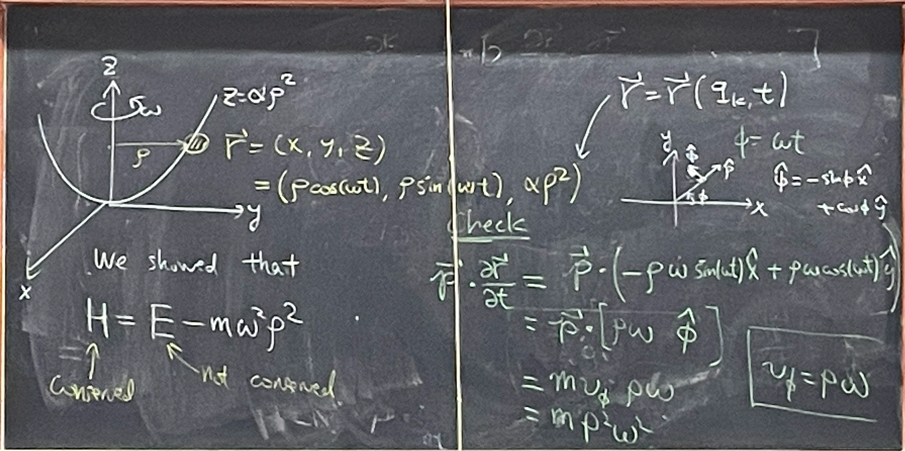
\includegraphics[scale=0.6]{July 3/july 3 pic 1.png}
\end{center}

\vskip 0.5cm
\begin{bluebox}
  If we break the force on the bead into a normal force (denoted $N$) and a centripetal(?) force, then

\begin{align*}
  dW &= \overbrace{N \rho}_{\text{torque about z-axis}} d\phi \\
  &= \frac{d {l}_z}{dt} d\phi \\
  &= d \left(\rho m \rho \omega\right) \omega \\
  &= d\left(m \rho^2 \omega^2\right)
\end{align*}

This is the energy that goes into the system.

\vskip 0.5cm
By energy conservation, $dW = dE$.
\begin{align*}
  \implies 0 = dE - dW = dE - d(m\rho^2 \omega^2)
\end{align*}

i.e. $E - m\rho^2 \omega^2 = H$ is a conserved quantity.
\end{bluebox}

\vskip 0.25cm
So, the \textbf{Hamiltonian being conserved} and the \textbf{Hamiltonian being equal to Energy} are two different scenarios with two different conditions.

\begin{redbox}
  \begin{itemize}
    \item The Lagrangian is time-independent i.e. $\frac{\partial L}{\partial t} = 0 \implies H$ is conserved. 
    \item The position vector centered in an inertial frame $\vec{r} = \vec{r}(q_k, t)$ is time independent i.e $\frac{\partial \vec{r}}{\partial t} = 0 \implies H = E$
  \end{itemize}
\end{redbox}

\vskip 0.5cm
Now we move on to a powerful technique.

\vskip 1cm
\subsection{The Method of Lagrange Multipliers}

\vskip 0.5cm
\begin{center}
  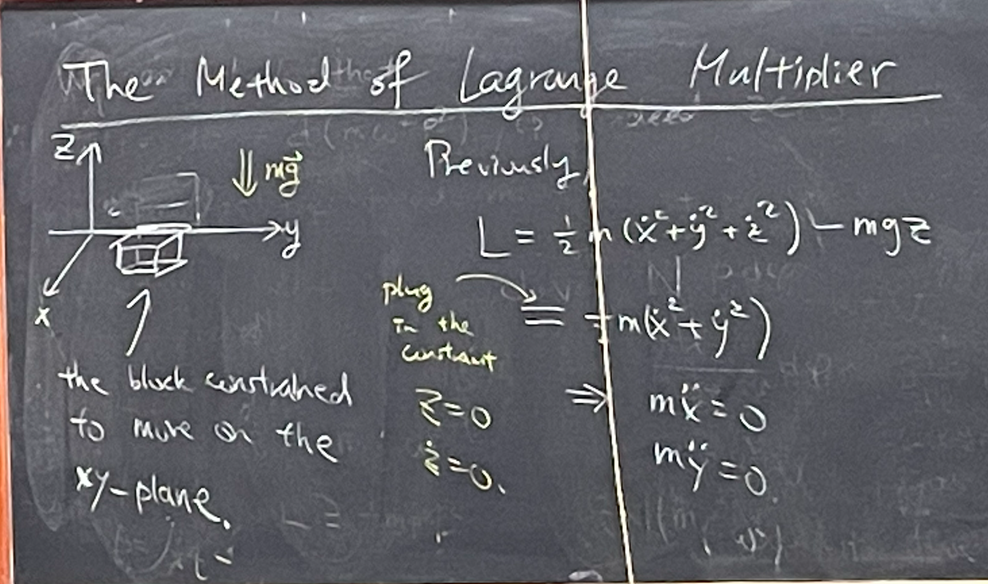
\includegraphics[scale=0.3]{July 3/july 3 pic 2 method of lagrange multipliers.png}
\end{center}

\vskip 0.5cm
We have a block constrained to move on the $xy$-plane, and we have gravity. Previously, we would say 
\[ L = \frac{1}{2} m \left( \dot{x}^2 + \dot{y}^2 + \dot{z}^2\right) - mgz \] i.e we would start with an unconstrained lagrangian, and then plug in the constraints $z = 0, \dot{z} = 0$
\begin{align*}
  &L = \frac{1}{2}m(\dot{x}^2 + \dot{y}^2) \\
  \implies & \begin{cases}
    m \ddot{x} = 0 \\
    m \ddot{y} = 0
  \end{cases} 
\end{align*}

\vskip 0.5cm
Alternatively, we can implement the constraint $\ddot{z} = 0$ in the following way: We have the original lagrangian
\begin{align*}
  L' = \frac{1}{2} m \left( \dot{x}^2 + \dot{y}^2 + \dot{z}^2\right) - mgz + \lambda z
\end{align*}

where $\lambda$ is the Lagrange multiplier and we can think of $z$ as being the constraint function $f(z)$ and our constraint is $f(z) = 0$.

\vskip 0.5cm
If we treat $\lambda$ as an independent degree of freedom, we can write the Euler-Lagrange equation for $\lambda$ as 
\[ \frac{\partial L}{\partial \lambda} - \frac{d}{dt} \left(\frac{\partial L}{\partial \dot{\lambda}}\right) = 0 \implies z = 0 \text{ (constraint)} \]

On the other hand, if we look at the equation of motion for $z$, we get 
\[  \frac{\partial L}{\partial z} - \frac{d}{dt} \left(\frac{\partial L}{\partial \dot{z}}\right) = 0 \implies \lambda - mg - m\ddot{z} = 0 \implies m\ddot{z} = \lambda - mg \]

and using the constraint $z = 0 \implies \ddot{z} = 0$ we get $-mg + \lambda = 0 \implies \lambda = mg$. Okay, but what physical meaning does $\lambda$ have? It has to do with the \textbf{Normal force}. i.e. $\lambda$ is encoding the \textbf{constraint} that the block can only move on the $xy$-plane due to the Normal force. 

\begin{redbox}
  So, in general, for $N$ constraints we have Lagrange Multipliers $\lambda_1, \cdots, \lambda_N$.
\end{redbox}

\begin{bluebox}
  \textbf{Why do we call $\lambda$ a Lagrange Multiplier?}
  \vskip 0.5cm
  Recall from Calc 3 that if we have contours of a function $f(x,y)$ on the $xy$-plane and we are constrained to move along some other curve $g(x,y) = c$ on the plane, if we ask 
  \color{blue}
  "What is the extremum of $f(x,y)$ as we move along the curve $g(x,y) = c$?"
  \color{black} then visually we can tell that the extremum corresponds to the point where $g(x,y)$ intersects the contour of $f(x,y)$ only once. This is because at such a point, the gradients of the two functions are parallel:

  \[ \nabla g = \lambda \nabla f \]
  This constant multiplier is the \textbf{Lagrange Multiplier}
\end{bluebox}

\begin{center}
  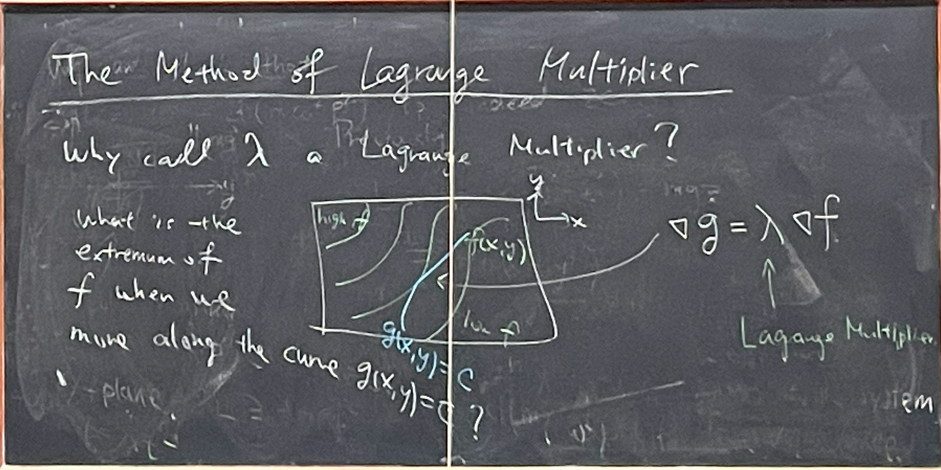
\includegraphics[scale=0.5]{July 3/july 3 pic 3 why do we call them lagrange multipliers.png}
\end{center}

So, in general, if we have a Lagrangian 
\[ L = \frac{1}{2}m \left(\dot{x}^2 + \dot{y}^2 + \dot{z}^2\right) - V(x,y,z) \]
we know that $\delta L = 0$ gives the Equations of Motion. But if we want to do this variation $\delta L$ under some constraint $C(x,y,z) = 0$ then we need to consider 
\[ \delta L = \lambda \delta C \implies L' = L - \lambda C \]


\vskip 0.5cm
\begin{redbox}
  Generally, if we have $P$ constraints, $C_{l}(q_1, \cdots, t) = 0$, $l = 1, \cdots, P$ on the lagrangian $L$, we can write a new lagrangian 
  \[ L' = L + \sum_{l = 1}^{P} \lambda_l C_l \]
  The Euler-Lagrange equation for $\lambda_l$ leads to $C_l = 0$ and the Euler-Lagrange equation for the generalized coordinate $q_k$ is 
  \[ \left( \frac{\partial L }{\partial q_{k}} - \frac{d}{dt} \left( \frac{\partial L}{\partial \dot{q}_{k}} \right) - \sum_{l = 1}^{P} \lambda_l \frac{C_l}{q_k} \right) = 0 \] 

  \begin{align*}
    \implies& \frac{d}{dt} \left( \frac{\partial L}{\partial \dot{q}_{k}} \right) = \frac{\partial L }{\partial q_{k}} + \underbrace{\sum_{l = 1}^{P} \lambda_l \frac{C_l}{q_k} }_{\text{generalized force}}
  \end{align*}
\end{redbox}

On the physical point of view, consider the following system:

\vskip 0.5cm
% [include picture of block and sledge which can both move]
\begin{center}
  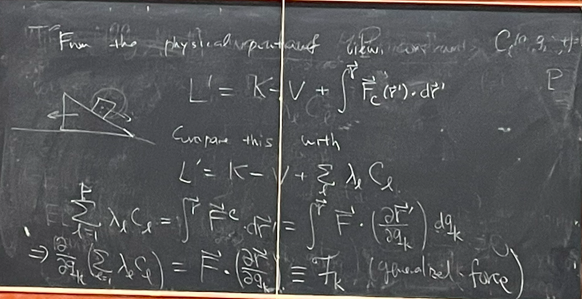
\includegraphics[scale=0.6]{July 3/july 3 pic 4 generalized force.png}
\end{center}
\vskip 0.5cm

If we consider the system as a whole, the normal forces due to the block and the sledge are equal and opposite, so they cancel each other out - and so does the work that they do(?).

\vskip 0.5cm
Howeverm if we consider the block only - we do have a normal force. The block is constrained the only move on the surface of the slope, so we can write 

\begin{align*}
  L' = K - V + \int^{\vec{r}} \vec{F}_C(\vec{r}) \cdot d\vec{r}'
\end{align*}

\begin{thought}
  {This is a bit handwavy - watch the lecture recording and think about this}
\end{thought}

Then, if we conpare this with 
\[ L' = L - V + \sum_{l} \lambda_l C_l \]

we have 
\begin{align*}
  &\sum_{l} \lambda_l C_l = \int^{\vec{r}} \vec{F}_C \cdot d\vec{r}' = \int^{\vec{r}} \vec{F} \cdot \left( \frac{\partial \vec{r}'}{\partial q_k} \cdot \mathrm{d}q_k \right) \\
  \implies& \frac{\partial}{\partial q_k} \left( \sum_{l} \lambda_l c_l \right) = \vec{F} \cdot \left( \frac{\partial \vec{r}}{\partial q_{k}} \right) \equiv \mathcal{F}_k \text{  (generalized force)}
\end{align*}

\hrule

\pagebreak
\section{July 8, 2024: Lagrange Multipliers}

\vskip 0.5cm
\subsection{More about Lagrange Multipliers}
Last time, we saw that if we have constraints $C_l \left(\underbrace{q_1, \cdots, q_k}_{N}, t\right) = 0$ then we can write a constrained Lagrangian
\[ L' = K - V + \sum_{l} \lambda_l C_l \]

These kinds of constraints, which are only constraints of the generalized coordinates are called \textbf{Holonomic constraints}. But these are not the most general constraints; we can have constaints which also depend on the derivatives $\dot{q_{k}}$. Those types of constraints are called \textbf{Non-holonomic constraints}.

Then, the principle of stationary action gives us 
\begin{align*}
  0 &= \delta S \implies \begin{cases}
    \frac{d}{dt} \left( \frac{\partial L}{\partial \dot{q_{k}}} \right) = \frac{\partial L}{\partial q_{k}} + \sum_{l} \underbrace{\lambda_l C_l}_{\vec{F}^C \frac{\partial \vec{r}}{\partial q_{k}} } \\
    C_l = 0
  \end{cases}
\end{align*}

\vskip 0.5cm
Note that there are multiple ways to write the same constraint. And writing a constraint in a different manner changes the $C_l$, which further changes the $\lambda_l$. As such, the $\lambda_l$ is not always a generalized force; it can also be a torque etc.

\vskip 0.5cm
In total we have $N+P$ variables and $N+P$ equations, so we are able to solve the system if we know the initial conditions.

\vskip 0.5cm
We got the above equation by varying the action, and in particular, by varying $L$ with respect to $q_k$. But we can extend this a bit futher\dots

\begin{align*}
  \begin{cases}
    \frac{d}{dt} \left( \frac{\partial L}{\partial \dot{q_{k}}}  \right)= \frac{\partial L}{\partial q_{k}} + \sum_{l} a_{lk} \lambda_{l} \\
    a_{lk} \delta q_{k} + a_{lt} \delta t = 0
  \end{cases}
\end{align*}
(Here, the $l$ index labels the \textbf{constraint} and the $k$ labels the coordinate.)

\begin{redbox}
  In the case of Holonomic constraint,
  \begin{align*}
    a_{lk} &= \frac{\partial C_l}{\partial q_{l}} \\
    a_{lt} &= \frac{\partial C_l}{\partial t} \\
  \end{align*}
\end{redbox}

\vskip 0.5cm
For Holonomic constraint, we will have 
\[ \frac{\partial q_{lk}}{\partial t} = \frac{\partial q_{lt}}{\partial q_{k}} \]








\subsection{Example: Tree log rolling down a ramp}

Consider a tree log rolling down a (fixed) ramp without sliding.
\vskip 0.5cm
[Include Figure]

\vskip 0.5cm
To describe the motion of the log, generically, we need two degrees of freedom: $X$ and $\theta$.

\vskip 0.5cm
But we also know the log is rolling \textbf{without sliding}. So if the tree moves a distance $dx$ during rotation $d\phi$, then we know $Rd\phi = dx$
where $R$ is the radius of the log. Or in other words,
\[ R d\phi - dx = 0 \]

\vskip 0.5cm
This constraint is of the general form we saw above: 
$ \boxed{a_{lk} \delta q_{k} + a_{lt} \delta t = 0 }$
with $a_{1,\theta} = R, a_{1, x} = -1$ and all the time components $a_{lt} = 0$.

\vskip 0.5cm
Now, we can write the Lagrangian of this system: 
\[ L = \frac{1}{2}M(\dot{X}^2) + \frac{1}{2}I \dot{\theta}^2 + mg X \sin(\alpha) \]

Note that we're actually kind of mixing approaches here. Technically there should be \emph{three} degrees of freedom because the log can move in $(x,y)$ space and rotate, but we know that the log is constrained by the Normal force and we don't need both of $x,y$; just one will suffice.

\begin{bluebox}
  \textbf{Wait... so, why do we even bother using the Lagrange Multiplier stuff if we're gonna use the old method too?} 

  \vskip 0.5cm
  The Lagrange multiplier method allows us to retain info about the contact forces so if we, say, want to find the magnitude of the tension in a string, we can still do so using the Lagrange Multiplier method. Whereas in the old method, contact forces are used to enfore constraints but we lose all information about them.
\end{bluebox}

\vskip 0.5cm
Anyway, after writing down the lagrangian, we can obtain the Equations of Motion (with the constraints):
\begin{align*}
  \begin{cases}
    \frac{d}{dt} \left( m\dot{X}\right) = +mg \sin(\alpha) - \lambda_1 \\
    \frac{d}{dt} \left( I \dot{\theta} \right) = \lambda_1 R
  \end{cases}
\end{align*}

\begin{redbox}
  \textbf{So, what exactly is $\lambda_1$? }
  \vskip 0.5cm
  In the $X$ equation of motion, we have $+mg\sin(\alpha)$ which is the component of gravity along the ramp. So, $\lambda_1$ has the same units as force. We can interpret $\lambda_1$ as the \textbf{frictional force}! 

  \vskip 0.5cm
  Then, in the $\theta$ equation of motion, we can interpret $\lambda_1 R$ as the \textbf{torque due to friction}!
\end{redbox}

Solving these further we have 
\begin{align*}
  \begin{cases}
    m \ddot{X} = mg\sin(\alpha) - \lambda_1 \text{ (1)}\\
    I \ddot{\theta} = \lambda_1 R \text{ (2)}\\
    R \dot{\theta} = \dot{X} \text{ (from the no-sliding condition)} \implies R \ddot{\theta} = \ddot{X} \text{ (3)}
  \end{cases}
\end{align*}

Substituting (3) into (1) gives

\begin{align*}
  &\begin{cases}
    mR \ddot{\theta} = mg \sin(\alpha) - \lambda_1 \\
    \frac{I}{R} \ddot{\theta} = \lambda_1
  \end{cases} \\ &\implies mR \left( \lambda_1 \frac{R}{I} \right) = mg\sin(\alpha) - \lambda_1 \\
  &\implies \left( 1 + \frac{mR^2}{I} \right) \lambda_1 = mg \sin(\alpha) \\
  &\implies \boxed{\lambda = \frac{mg \sin(\alpha)}{\left(1 + \frac{mR^2}{I}\right)}} \text{ This is the magnitude of friction!}
\end{align*}

\vskip 1cm
\subsection{Example: A bead on a wire}

\vskip 0.5cm
We've seen this example before, but this time we want to calculate the normal force on the bead.

\vskip 0.5cm
[Include Figure]

\vskip 0.5cm
Using the Lagrange Multiplier method, we can write down the constrained Lagrangian as 
\[ L' = \frac{1}{2}m \left[ \dot{\rho}^2 + \rho^2 \dot{\phi}^2 + \dot{z}^2 \right] -mgz - \lambda_1 \left(\phi - \omega t\right) - \lambda_2 \left(z - \alpha \rho^2\right) \]

So, the EL Equations look like 

\begin{align*}
  \begin{cases}
    m \ddot{\rho} = n\rho \dot{\phi}^2 - 2 \lambda_2 \alpha \rho \\
    \frac{d}{dt} \left( m \rho^2 \dot{\phi} \right) = \lambda_1 \\
    m \ddot{z} = -mg + \lambda_2 
  \end{cases}
\end{align*}

\vskip 0.5cm
\begin{redbox}
  From the $z$ EoM, we can tell that $\lambda_1$ is a force since it's being added with $-mg$. We can interpret it as the \textbf{$z-$component} of the \textbf{Normal Force}.

  \vskip 0.5cm
  Similarly, in the $\phi$ EoM we see that $\lambda_1$ is the derivative of the Angular Momentum, so $\lambda_1$ is the \textbf{torque}.
\end{redbox}

[Include figure]

\begin{redbox}
  Now, in the $\rho$ equation, we know that $m\ddot{\rho}$ is also a force since $\rho$ has units of length. So, $-2\lambda_2 \alpha \rho$ must also be a force. Exactly which force is it? It's the \textbf{radial component} of the \textbf{Normal Force} (See the figure above.)
\end{redbox}

\vskip 0.5cm
\begin{bluebox}
  When it comes to actually solving for $\lambda_1$ and $\lambda_2$, we can solve for them after we solve for $\rho(t)$ using $z = \alpha \rho^2$ and other constraints.
\end{bluebox}

\vskip 0.5cm
[Add last bit from lecture recording - lots of figures]
\hrule

\pagebreak
\section{July 9, 2024: Symmetries and Lagrangians}

\subsection{Note about the discussion from last time}
[Write about clever method to find rolling constraint that Chien-I spoke about at the beginning of lecture]

\vskip 0.5cm
\subsection{Symmetries}
Previously we discussed \textbf{Cyclic Coordinates}: 
\begin{redbox}
  A coordinate $q_{k}$ is cyclic if 
  \[ \frac{\partial L}{\partial q_{k}} = 0\]
  As a result, the EL equation gives us the result that 
  \[ p_{k} \equiv \frac{\partial L}{\partial \dot{q_{k}}} \text{ is conserved} \]
\end{redbox}

\begin{bluebox}
  This is a \textbf{symmetry} in the sense that when we change $q_{k}$, the Lagrangian does not change.
\end{bluebox}

\vskip 0.5cm
\textbf{What exactly is a Symmetry?}
We define a symmetry of a system to be a \textbf{transformation} of the system such that the system behaves the same after transformation. For example, rotating a triangle by $120$ degrees is a symmetry transformation of the triangle.

\vskip 0.5cm
The study of symmetries falls under \textbf{Group Theory}, but in physics we're usually concerned specifically \textbf{continuous transformations}. Continuous symmetries often give rise to \textbf{conserved quantities}.

\begin{redbox}
  \textbf{Example:} $\theta$ independent lagrangian
\end{redbox}

We'll see this in more detail when we study Noether's Theorem.

\vskip 0.5cm
\subsection{Continuous Transformations}
Usually, we have $L = L\left(q_{k}, \dot{q}_{k}, t\right)$. We can apply transformations on the $q_{k}$ and $t$ variables
\begin{align*}
  q_{k} &\rightarrow q'_{k}(q_{k}, t) \\
  t &\rightarrow t'(t) \\
\end{align*}
which in turn transform the lagrangian $L$

\vskip 0.5cm
When we say a transformation is continuous, we mean that we can make a transformation parametrized by some small parameter $\epsilon$ such that when $\epsilon \rightarrow 0$, the transformation is just the identity transformation.

\vskip 0.5cm
Since the mapping is continuous, we can expand the transformation as 
\begin{align*}
  q_{k}(t) &\rightarrow q'_k(t') = q_{k}(t) + \delta q_{k} \\
  t &\rightarrow t(t) = t + \delta t \\
\end{align*}

\begin{redbox}
  \textbf{Example: Continuous Rotation}
  In the plane $\mathbb{R}^2$, we can rotate a vector $V = V_x \hat{x} + V_y \hat{y}$ using a standard rotation matrix:
  \[ \vec{V} \rightarrow \vec{V}' = \begin{pmatrix}
    \cos(\theta) & -\sin(\theta) \\
    \sin(\theta) & \cos(\theta) 
  \end{pmatrix} \begin{pmatrix}
    V_x \\
    V_y
  \end{pmatrix} \]
  where $\theta$ is a continuous parameter that represents the angle of rotation.
\end{redbox}

\begin{redbox}
  \textbf{Examples: Non-continuous transformation}
  \begin{enumerate}
    \item Dicrete rotation: Rotations where $\theta$ is only allowed to have specific values, for example $\theta =  n \frac{\pi}{6}$
    \item Parity: $(x,y,z) \rightarrow (-x,-y,-z)$
  \end{enumerate}
\end{redbox}

\vskip 0.5cm
There are two ways to generate transformations in $q_{k}$. 
\begin{enumerate}
  \item With a fixed time, we can "mix" the coordinates:
  \[ q_{k}(t) \rightarrow q_{k}'(t) = q_{k}(t) + \underbrace{\Delta q_{k}(t) }_{\text{small transformation}} \]

  For example, we can rotate a vector without messing with the time coordinate:
  \begin{align*}
    \begin{pmatrix}
      x'(t) \\
      y'(t)
    \end{pmatrix} = \begin{pmatrix}
      1 & -\theta \\
      \theta & 1
    \end{pmatrix} = \begin{pmatrix}
      x(t) - \theta y(t) \\
      y(t) + \theta x(t) 
    \end{pmatrix}
  \end{align*}

  We can represent this transformation concisely using the \textbf{levi-civita symbol, $\epsilon_{ij}$}
  \[ \boxed{x_i' = x_i - \theta \epsilon_{ij}x_j } \]

  \vskip 0.5cm
  \item We can generate a change in $q_{k}$ by shifting the time: $t \rightarrow t + \delta t(t)$
  \[ q_{k}(t) \rightarrow q_{k}(t') = q_{k}(t + \delta t) = q_{k}(t) + \dot{q}_{k} \delta t \]
\end{enumerate}

\vskip 0.5cm
We can define the total (infinitessimal) transformation of $q_{k}$ as 
\begin{align*}
  \delta q_{k} &\equiv q_{k}'(t') - q_{k}(t) = q_{k}'(t + \delta t) - q_{k}(t) \\
  &\approx q_{k}'(t) + \dot{q}_{k}' \delta t = q_{k}(t) \\
  \text{to first order $\rightarrow$  } &\approx q_{k}(t) + \Delta q_{k}(t)\dot{q}_{k}(t) \delta - q_{k}(t)
\end{align*}
where we used 
\[ \dot{q}_{k}'(t) = \frac{d}{dt} \left( q_{k} + \Delta q_{k} \right) = \dot{q}_{k}(t) + \frac{d}{dt} \left(\Delta q_{k}\right) \]

\vskip 0.5cm
Thus, to first order, we have 
\[ \boxed{\delta q_{k}(t) = \Delta q_{k}(t) + \dot{q}_{k} \delta t} \]

\vskip 0.5cm
\begin{bluebox}
We say such a transformation by $\delta q_{k}$ and/or $\delta t$ is a symmetry if we have the same dynamics i.e. under the transformation, the \textbf{action, $\delta S = 0$} does not change.  ($\delta S$ is the change in $S$ when we perform a particular transformation in terms of $\Delta q_{k}$ and/or $\delta t$)
\end{bluebox}

\vskip 0.5cm
\begin{align*}
  0 &= \delta \left( \int dt L(q_{k}, \dot{q}_k, t)\right) \\
  &= \int \delta(dt) L + \int dt \delta L \\
  &= \int dt \color{blue}\frac{d(\delta t)}{dt} L \color{black} + \int dt \left( \color{red} \frac{\partial L}{\partial q_{k}} \delta q_{k} + \frac{\partial L}{\partial \dot{q}_{k}} \frac{d}{dt}( \Delta q_{k} ) \color{black} + \color{blue} \frac{dL}{dt} \delta t \color{black} \right)
\end{align*}
\vskip 0.5cm
where we should note that $dL/dt$ is the \textbf{total} derivative
\[ \frac{dL}{dt} = \frac{\partial L}{\partial q_{k}} \dot{q}_k  + \frac{\partial L}{\partial \dot{q}_{k}} \ddot{q}_k + \frac{\partial L}{\partial t} \]

\vskip 0.5cm
Continuing on and applying "Integration by Parts",
\begin{align*}
  0 &= \int dt \left[ \color{red} \left( \frac{\partial L}{\partial q_{k}} - \frac{d}{dt} \left( \frac{\partial L}{\partial \dot{q}_k} \right) \right) \Delta q_{k} + \frac{d}{dt} \left( \frac{\partial L}{\partial \dot{q}_{k}} \Delta q_{k} \right) \color{black} + \color{blue}\frac{d}{dt} \left( L \delta t \right) \color{black} \right]
\end{align*}

\vskip 0.5cm
If $q_k$ satisfies the EoM,
\begin{align*}
  0 &= \int_{t_i}^{t_f} dt \left[ \frac{d}{dt} \left( \frac{\partial L}{\partial \dot{q}_{k}} \Delta q_{k} + L \delta t\right) \right] = \left[ \frac{\partial L}{\partial \dot{q}_k} \Delta q_{k} + L \delta t \right]_{t_i}^{t_f}
\end{align*}

Therefore the quantity
\[ Q \equiv \frac{\partial L}{\partial \dot{q}_k} \Delta q_{k} + L \delta t  \]
is conserved! What we've shown is Noether's Theorem.

\vskip 0.5cm
\begin{bluebox}
  \underline{\textbf{Noether's Theorem:}}
  If we have a continuous symmetry and the evolution of the system satisfies the EoM, then there is an associated conserved quantity given by 
  \[ Q \equiv \frac{\partial L}{\partial \dot{q}_k} \Delta q_{k} + L \delta t  \]
  which is called the \textbf{Noether Charge}.
\end{bluebox}

\vskip 0.5cm 
In fact, we can extend this a little bit. The action can change, as long as it's of the form:
\[ \delta S = \int dt \left( \frac{dK}{dt} \right) \]
because such a change just adds constant boundary terms $K(t_f) - K(t_i)$ which do not change the dynamics. So,
\[ \frac{d}{dt} \left( Q - K \right) = 0 \]

\vskip 0.5cm
This $Q - K$ is a more general conserved charge.

\vskip 0.5cm
\subsection{Example: Spacial Translation}
\[ L = \frac{1}{2} m\dot{x}^i \dot{x}_i \]
This Lagrangian is invariant under the shift $\begin{cases}
  x_i \rightarrow x_i + \epsilon_i \text{  spatial translation} \\
  t \rightarrow t \text{ no time translation}
\end{cases}$. 

So, $\delta x_i = \Delta x_i + \dot{x} \underbrace{\delta t}_{=0}$. As a result,

\[ Q \equiv \frac{\partial L}{\partial \dot{x}_i} \Delta x_i = m\dot{x}_i \epsilon_i \implies m\dot{x}_i \text{ is conserved.}\]

\vskip 0.5cm
\subsection{Example: Time Translation}
Consider the time translation 
\[ \begin{cases}
  x_i \rightarrow x_i \\
  t \rightarrow t + \delta t
\end{cases}  \]
i.e. $\delta x_i = 0 = \Delta x_i + \dot{x}_i \delta t$ which implies 
\[ \Delta x_i = -\dot{x}_i \delta t \]

\vskip 0.5cm
Consider the following Lagrangian under time translation
\[ L = \frac{1}{2}m\dot{x}^i \dot{x}_i - V(x) \]

Since $L = L(x_i, \dot{x}_i, t)$, if the $x_i$'s don't change then the change in $L$ is just 
\begin{align*}
  \delta L &= \frac{\partial L}{\partial x_i} \underbrace{\delta x_i}_{=0} + \frac{\partial L}{\partial \dot{x}_i} \underbrace{\delta dot{x}_i}_{=0} + \frac{\partial L}{\partial t} \delta t \\
  &= \frac{\partial L}{\partial t} \delta t  
\end{align*} 

\vskip 0.5cm
And, when $ \frac{\partial L}{\partial t} \delta t  = 0$, we have time translation symmetry, giving us the conserved current

\begin{align*}
  Q &\equiv  \frac{\partial L}{\partial \dot{x}_i} \delta x_i + L \delta t \\
  &= -  \frac{\partial L}{\partial \dot{x}_i} \dot{x}_i \delta t  +  L \delta t \\
  &= \left(  \frac{\partial L}{\partial \dot{x}_i} \dot{x}_i - L \right) \left(- \delta t\right)
\end{align*}

\vskip 0.5cm
\begin{bluebox}
So when we have time translation symmetry, the \textbf{Hamiltonian}
\[ H =  \frac{\partial L}{\partial \dot{x}_i} \dot{x}_i - L  \]
is conserved.
\end{bluebox}

\vskip 0.5cm
\subsection{Example: Isotropic Harmonic Oscillator under rotation}
Consider 
\[ L = \frac{1}{2}m \dot{x}^i \dot{x}_i - \frac{1}{2}k x^i x_i \]
under rotation
\begin{align*}
  x_i &\rightarrow x_i - \theta \epsilon_{ij} x_j \\
  t \rightarrow t
\end{align*}

Then, the Lagrangian transforms into 
\begin{align*}
  L &\rightarrow \frac{1}{2}m \dot{x}^i \dot{x}_i - \frac{1}{2}k x^i x_i + m\dot{x}_i \left(-\theta \epsilon_{ij} \dot{x}_j\right) - kx_i \left(-\theta \epsilon_{ij} x_j\right) + \mathcal{O}(\epsilon^2) \\
  &= L - \theta m \epsilon_{ij} \dot{x}_i \dot{x}_j + k \epsilon_{ij} x_{i} x_{j} \\
  &= L
\end{align*}

where we used the fact that $\epsilon_{ij}$ is antisymmetric while $\dot{x}_i \dot{x}_j$, $x_i, x_j$ are antisymmetric. Thus, 
the two terms other than $L$ vanish.

\begin{redbox}
  In general if we have 2-d tensors $S_{ij} = S_{ji}$ (symmetric) and $A_{ij} = -A_{ji}$ (antisymmetric) then 
  \begin{align*}
    S_{ij} A_{ij} &= -S_{ij} A_{ji} \\
    &= -S_{ji} A_{ji} \\
    &= -S_{ij} A_{ij} \text{ Since $S_{ij} A_{ij}$ is itself symmetric as a whole} \\
    \implies S_{ij} A_{ij} &= 0
  \end{align*}
\end{redbox}

\vskip 0.5cm
Here, the conserved current is 
\begin{align*}
  Q &\equiv \frac{\partial L}{\partial \dot{x}_i} \Delta x_i \\
  &= m \dot{x}_i \left(-\theta \epsilon_{ij} x_{j}\right) \\
  &= -\theta \epsilon_{ij} x_j m\dot{x_i} \\
  &= -\theta \epsilon_{12} x_2 m\dot{x}_1 - \theta \epsilon_{21} x_1 m \dot{x}_2 \text{  (The terms with $i=j$ vanish because $e_{ii} = 0$)} \\
  &= -\theta(ym\dot{x} - xm\dot{y}) 
\end{align*}
which implies that \textbf{Angular momentum is conserved.} This marks the end of today's lecture.
\hrule

\vskip 1cm.
\begin{note}
{No lectures on July 10, 11 because of the midterm.}
\end{note}


\pagebreak
\section{July 15, 2024: Obtaining Lagrangians from Symmetries}

Today, we wrap up our discussion of Lagrangians. The goal today is to find the most general Lagrangian $L(x, \dot{x}, t)$ describing a 1D system which is \textbf{time-translation invariant} and \textbf{Galilean invariant}.


% \vskip 0.5cm
The framework we'll develop is what's done a lot in research (eg. in Effective Field Theory research), where we consider the symmetries we must enforce and then find the most general possible Lagrangian.

\vskip 0.5cm
Also recall that a Lagrangian is called time-translation invariance if it has no eplicit time dependence. 

\vskip 0.5cm
\textbf{\underline{Step 1:}} Consider the action
\[ S = \int \mathrm{d}t L(x, \dot{x}, t) \]
and the Galilean transformation $x \rightarrow x + \Delta x = x - Vt$ ($V$ is a constant) which causes the variation
\vskip 0.5cm
\begin{align*}
  \delta S &= \int \mathrm{d}t \left[ \frac{\partial L}{\partial x}(-Vt) + \frac{\partial L}{\partial \dot{x}}(-V) \right] \\
  &= \int \mathrm{d}t \left[ (-V)\frac{d \Tilde{K}}{dt} \right]  \text{ (for some function $\Tilde{K}$)} \\
\end{align*}

(as long as the change in action is of the form above, there is no change in dynamics.)

\[ \implies \frac{\partial L}{\partial x} t + \frac{\partial L}{\partial \dot{x}} = \frac{d \Tilde{K}}{dt} = \frac{\partial \Tilde{K}}{\partial x} \dot{x} +  \frac{\partial \Tilde{K}}{\partial \dot{x}} \ddot{x} + \frac{\partial \Tilde{K}}{\partial \ddot{x}} \dddot{x} + \cdots +  \frac{\partial \Tilde{K}}{\partial t}  \\ \]

\vskip 0.5cm
But the LHS has derivatives up to $\dot{x}$ at most since we restrict our lagrangians. So, we must have $\Tilde{K} = \Tilde{K}(x, t)$ and 
\[ \frac{\partial L}{\partial x} t + \frac{\partial L}{\partial \dot{x}} = \frac{\partial \Tilde{K}}{\partial x} \dot{x} + \frac{\partial \Tilde{K}}{\partial t} \;\;\;\;\;\;\;\;\; (\star)\]

\vskip 0.5cm
\textbf{\underline{Step 2:}} Notice is that $\Tilde{K} = \Tilde{K}(x, t)$ means that the only place in equation $(\star)$ that we have $\dot{x}$-dependence is $ \frac{\partial \Tilde{K}}{\partial x} \dot{x} + \frac{\partial \Tilde{K}}{\partial t}$ i.e. it is linear in $\dot{x}$.
\vskip 0.5cm
$\implies$ at most, $L$ can only be second order in $\dot{x}$, namely
\[ L = f_2(x,t) \dot{x}^2 + f_1(x,t) \dot{x} + f_0(x, t) \]

\textbf{\underline{Step 3:}} Finally, if we enfore time-translation symmetry then we have 
\[ \frac{\partial L}{\partial t} = 0  \]
which tells us $f_i(x, t) = f_i(x)$ and so,
\[ \implies L = f_2(x) \dot{x}^2 + f_1(x) \dot{x} + f_0(x) \;\;\;\;\;\;\;\; (\Delta) \]

\textbf{\underline{Step 4:}} Let's look at equation $(\star)$ again, which we obtained from enforcing Galilean invariance. With $(\Delta)$ we know 
\[ \frac{\partial L}{\partial x} \supseteq \frac{\partial f_2}{\partial x} \dot{x}^2 \]

(sidenote: this is an abuse of notation that I love; it literally just means that $\frac{\partial L}{\partial x}$ includes a term $\frac{\partial f_2}{\partial x} \dot{x}^2$ it's so goofy fr)

But the RHS of equations $(\star)$ has no $\dot{x}^2$ terms. Thus,
\[ \frac{\partial f_2}{\partial x} = 0 \] i.e. $f_2$ is a constant.

\vskip 0.5cm
\textbf{\underline{Step 5:}} For the $f_1(x) \dot{x}$ term in the Lagrangian, we can say 

\[ S \supseteq \int_{i}^{f} f_1(x) \dot{x} dt = \int_{i}^{f} f_1(x) dx = F(x_f) - F(x_i) \text{ (constant)}\] so this does not affect the dynamics and so we can safely throw it out of the Lagrangian and shove it to the curb.

\vskip 0.5cm
\textbf{\underline{Step 6:}} The only thing left is 
\[ L = f_2 \dot{x}^2 + f_0(x) \]

Plugging this back into equation $(\star)$, we get 

\begin{align*}
  \frac{\partial L}{\partial x} t + \frac{\partial L}{\partial \dot{x}} &= \frac{\partial \Tilde{K}}{\partial t} + \frac{\partial \Tilde{K}}{\partial x} \dot{x} \\
  \implies \frac{\partial f_0}{\partial x} t + 2 \dot{x} f_2 &= \frac{\partial \Tilde{K}}{\partial t} + \frac{\partial \Tilde{K}}{\partial x} \dot{x} \;\;\;\;\;\;\;\;\;\;\; (\square)
\end{align*}

Matching the terms with and without $\dot{x}$ dependence, we get
\begin{align*}
   \frac{\partial \Tilde{K}}{\partial x} = 2f_2 = \text{ constant} \implies \Tilde{K} = 2f_2 x + g(t)
\end{align*}

\vskip 0.5cm
\textbf{\underline{Step 7:}} 
Plugging the expression for $\Tilde{K}$ into equation $(\square)$ we get 

\begin{align*}
  \frac{\partial f_0}{\partial x} t + 2\dot{x}f_2 = \frac{\partial g}{\partial t} + 2f_2 x &= \frac{\partial g}{\partial t} + 2f_2 \dot{x} 
\end{align*}

but $g(t)$ has no $x$-dependence $\implies \frac{\partial f_0}{\partial x}$ cannot have $x$-dependence 
\[ \implies f_0 = c_1x + c_0 \]

\begin{bluebox}
  In summary, the most general Lagrangian for a 1D particle that is time-translation invariant and Galilean invariant is of the form 
  \[ L = c_2 \dot{x} + c_1 x + c_0 \]
  (where instead of writing $f_2$ we just wrote $c_2$). But also, constants don't affect the dynamics. Therefore, the most general Lagrangian we need is 
  \[ L = c_2 \dot{x}^2 + c_1 x \]
\end{bluebox}

\begin{redbox}
  \textbf{What kind of physics does this lagrangian describe?} 
  \vskip 0.25cm
  That of a non-relativistic particle subject to a constant force field. For example, if the field is that of uniform gravity, then 
  \[ L = \frac{1}{2}m\dot{x}^2 - mgx \]
\end{redbox}

\vskip 0.5cm
\begin{thought}
  {When people do this in Effective Field Theory, there are much more complicated symmetries to enfore such as $U(1), SU(2)$ etc. but the procedure is follows the same basic idea we've studied here.}
\end{thought}

\vskip 0.5cm
We were able to get a very specific form for our Lagrangian, but often symmetries are not strong enough to constrain our Lagrangian. In that case, we have to use other methods to determine the form of the Lagrangian for our system such as by experimental considerations.

\vskip 0.5cm
Okay, now we go back to some more tradition stuff from classical mechanics. 

\vskip 1cm
\subsection{Central Force Problem}

A \textbf{Central Force} is one whose potential energy function has \textbf{Spherical symmetry} eg. Isotropic Harmonic Osciallators or a particle under uniform gravitational force.

\vskip 0.5cm
Usually, we have a two-body problem with a Lagrangian of the form 

\[ L = \frac{1}{2} m_1 \dot{\vec{r}}_1^2 + \frac{1}{2} m_2 \dot{\vec{r}}_2^2 - U(r)\]
where $r = |\vec{r}_2 - \vec{r}_1|$. But, we can effectively change this into a one-body problem by using the \textbf{Center-of-Mass} coordinates.

\[ \vec{r} \equiv \vec{r}_2 - \vec{r}_1,\;\;\;\; \vec{R} \equiv \frac{m_1\vec{r}_1 + m_2 \vec{r}_2}{m_1 + m_2}  \]

Using these coordinates and $M \equiv m_1 + m_2$, $\mu = \frac{m_1m_2}{m_1 + m_2}$ we can write the Lagrangian as 

\[ L = \underbrace{\frac{1}{2} M \dot{\vec{R}}^2}_{\text{free motion of C.M.}} + \underbrace{\frac{1}{2}\mu \dot{\vec{r}}^2 - U(\vec{r})}_{\text{non-trivial dynamics}} \]

We've essentially decoupled the two bodies. Now, if $U(\vec{r})$ has spherical symmetry i.e. $U(\vec{r}) = U(r)$ then it is natural to work in spherical coordinates.

So, the non-trivial part of the Lagrangian will be 

\[ L = \frac{1}{2} \mu \left(\dot{r}^2 + r^2 \dot{\theta}^2 + r^2 \sin^2(\theta) \dot{\phi}^2 \right) - U(r) \]

and $\phi$ is a cyclic coordinate of it. Thus,
\[ p_{\phi} = \frac{\partial L}{\partial \dot{\phi}} = \mu r^2 \sin^2(\theta) \equiv l_z \] is conserved. Then,
\begin{align*}
  L &= \frac{1}{2} \left(\dot{r}^2 + r^2 \dot{\theta}^2 + \frac{l_z}{\mu^2 r^2 \sin^2(\theta)}\right) - U(r)
\end{align*}

\vskip 0.5cm
The fact that the angular momentum $l_z$ (and in fact, the \emph{total} angular momentum $l$) is conserved means that the particle is moving on a fixed plane.

\begin{redbox}
  \textbf{Why is total angular momentum conserved?}
  A central force cannot cause torque, therefore angular momentum is conserved.
\end{redbox}

WLOG, we set the $z-axis$ to be perpendicular to the motion of the plane i.e. we set $\theta = \frac{\pi}{2} \implies \dot{\theta} = 0$ due to which $\sin(\theta) = 1$. So, our non-trivial Lagrangian is 

\[ L = \frac{1}{2}\mu \dot{r}^2 + \frac{l_z}{2\mu r^2} - U(r) \]

Before we put the constraint on $\phi$, the Lagrangian is 
\[ L = \frac{1}{2}\mu \dot{r}^2 + \frac{1}{2} \mu r^2 \dot{\phi}^2 - U(r) \] and the corresponding Hamiltonian is
\begin{align*}
  H &= \frac{\partial L}{\partial \dot{q}_k} \dot{q}_k - L \\
  &= \frac{1}{2}\mu\dot{r}^2 + \frac{1}{2}\mu r^2\dot{\phi}^2 + U(r) \\
  &= \frac{1}{2} \mu \dot{r}^2 + \underbrace{\frac{l_z^2}{2\mu r^2} + U(r)}_{\text{effective potential}}
\end{align*}

Also, when we switch from Spherical Coordinates to Cartesian Coordinates we use 
\[ \begin{cases}
  x = r\sin\theta\cos\phi \\
  y = r\sin\theta\sin\phi \\
  z = r\cos\phi \\
\end{cases} \]
which have no time dependence, and so $H = E$. Aaaaaand... we're out of time so w'll continue tomorrow.


\pagebreak
\section{July 16, 2024: Central Forces and Orbital Shapes}

\subsection{Continuing our discussion of Central Forces}

As we saw last time, when dealing with a 2-body central force, we can do a \textbf{change of coordinates} to make things simpler.

\vskip 0.5cm
The dynamics of two bodies moving in a central force can be decoupled into the dynamics of a free body (moving with constant mass) and another mass subject to an effective potential.

\vskip 0.5cm
[Include figure of 1-body and 2-body central forces] 

[Write about the 2-body lagrangian being split into free and non-trivial parts.]

\vskip 0.5cm
\subsection{Aside: Ineratial Mass and Gravitational Mass}

In Newton's Law of Gravitation,
\[ |\vec{F}| = \frac{G \mu_1 \mu_2}{r^2} \]
the quantities $\mu_1, \mu_2$ are called gravitational mass (though a better name would be gravitational charge since the force is of the same form as coulomb's law). They tell us how strong thee interaction is.

\vskip 0.5cm
And, in Newton's First Law,
\[ |\vec{F}| = m|\vec{a}| \]
the term $m$ is the inertial mass. It tells us how hard it is to change the particles velocity.

\vskip 0.5cm
Now, a priori, there is no reason for these quantities to be the same. However, if we conduct an experiment where a base-ball and a feather free-fall towards the earth, we know

\begin{align*}
  a_{\text{baseball}} &= \frac{|\vec{F}|}{m_{\text{baseball}}} = \frac{G \mu_{\oplus} \mu}{R_{\oplus}^2 m_{\oplus}} \\
  a_{\text{feather}} &= \frac{|\vec{F}|}{m_{\text{feather}}} = \frac{G \mu_{\oplus} \mu}{R_{\oplus}^2 m_{\oplus}} \\
\end{align*}

and we find via the experiment that $a_{\text{baseball}} = a_{\text{feather}} = g$

Then, 
\begin{align*}
  \left( \frac{G \mu_{\oplus}}{R_{\oplus}^2} \right) \left(\frac{\mu_{\text{baseball}}}{m_{\text{baseball}}}\right) &= \left( \frac{G \mu_{\oplus}}{R_{\oplus}^2} \right) \left(\frac{\mu_{\text{feather}}}{m_{\text{feather}}}\right)
\end{align*}

So the gravitational mass to the inertial mass ratio is the same across objects! Note that $\mu/m$ is analogous to $e/m$ in electrostatics and, for example, the proton $p^+$ and electron $e^-$ has \emph{very different $e/m$ ratio}. But miraculously, when it comes to gravity, $\mu / m$ is the same for all objects. Numerically, we can just set $\mu$ and $m$ equal to each other. 


\begin{bluebox}
  The statement that $\mu / m$ is the same for all objects is called the \textbf{Equivalence Principle}. This has important implications in General Relativity.
\end{bluebox}

\begin{redbox}
  Include discussion about curved space and hockey pucks on the earth.
\end{redbox}

\subsection{Continuing on with the 2-body problem}

Focusing on the dynamics of $\vec{r}$, the Lagrangian for that part is 

\begin{align*}
  L &= \frac{1}{2}\mu \dot{\vec{r}}^2 - U(r) \\
  &= \frac{1}{2} \left( \dot{r}^2 + r^2 \dot{\theta}^2 + r^2 \sin^2(\theta) \dot{\phi}^2 \right) - U(r)
\end{align*}

But notice that these dynamics are the same as those of the 1-body central force scenario as $\vec{L}$ is conserved and motion is on a plance. i.e. $\theta$ is fxed which we can WLOG set to $\pi/2$.

\begin{align*}
  L &= \frac{1}{2} \mu \left( \dot{r}^2 + r^2 \dot{\phi}^2 \right) - U(r) \\
  \implies H &= \frac{1}{2} \mu \left(\dot{r}^2 + r^2 \dot{\phi}^2\right) + U(r) \\
  &= \frac{1}{2} \mu \dot{r}^2 + \underbrace{\frac{l_z^2}{2\mu r^2} + U(r)}_{\text{effective potential for a 1D d.o.f. } r, U_{\text{eff}}}
\end{align*}

This is where we stopped last lecture. The position $r$ is then subject to a force 
\begin{align*}
  F &= - \frac{\partial U_{\text{eff}}}{\partial r} \\
  &= +\frac{l_{z}^{2}}{\mu r^2} - \frac{\partial U(r)}{\partial r}
\end{align*}

where 
\[ \frac{l_{z}^{2}}{\mu r^2} =\frac{\mu^2r^2\dot{\phi}^2}{\mu r^2} = \frac{\mu v^2}{r} = \mu a_{c} \]

\vskip 0.25cm
This looks like a "centrifugal force".

\begin{redbox}
  Let's think about centrifugal forces for a sec. Consider the following setup where Bob is at a distance $r$ from the z-axis and is rotating about the axis a constant rate.

  \vskip 0.5cm
  [Include figure]
  \vskip 0.5cm

  In Bob's Frame, these three forces [complete this later]
\end{redbox}

\vskip 0.5cm
[Include figure of spring extending from fixed point]


\vskip 0.5cm
The angular momentum conservation keeps to $r$ to be non-zero because when $r = 0$, we have $l_z = 0$. This is why we have a positive sign in front of the $(l_z)^2 / \mu r^2$ term - the force is pushing outwards.


\vskip 0.5cm
This $U_{\text{eff}}$ also allows us to understand whether $r$ is a fixed value or changes between some $r_{\text{min}}$ and $t_{\text{max}}$. For example, if we consider a spring with $U(r) = \frac{1}{2} kr^2$ we get 

\[ U_{\text{eff}} = \frac{(l_z)^2}{2\mu r^2} + \frac{1}{2} kr^2 \]

Plotting this, we have
[Include figure]


[Write the discussion about the plot based on lecture recording and textbook.]

\vskip 0.5cm
If we instead consider a gravitational system with $U(r) = -\frac{G m_1 m_2}{r^2}$ we have 
\[ U_{\text{eff}} = \frac{(l_z)^2}{2\mu r^2} - \frac{Gm_1m_2}{r^2} \] which gives us the plot 

\vskip 0.5cm
[Include figure]

\vskip 0.5cm
You've probably seen a very similar plot when studying Chemistry/Quantum Mechanics. The reason for that is because the effective potential for an atom with $l \neq 0$ has a very similar form.

\vskip 0.5cm
[Include discussion of the plot based on lecture recording and textbook.]

\vskip 0.5cm
If we want to find $r(t)$ we can use 
\begin{align*}
  E &= \frac{1}{2} \mu \left(\frac{dr}{dt}\right)^2 + \frac{(l_z)^2}{2\mu r^2} + U(r) \\
  \implies \left(\frac{dr}{dt}\right)^2 &= \frac{2}{\mu} \left[ E - \frac{(l_z)^2}{2\mu r^2} - U(r) \right] \\
  \implies \int_{t_{0}}^{t} dt' &= \pm \sqrt{\frac{\mu}{2}} \int_{r_{0}}^{r} \frac{dr}{ \sqrt{E - \frac{(l_z)^2}{2\mu r^2} - U(r) }}
\end{align*}

and then after integrating, the inverse relation gives us $r(t)$.

\vskip 1cm
\subsection{Orbital Shape}
We will just to pure 1-body problems here, but the procedure remains the same (just more tedious) in the 2-body case.

\vskip 0.5cm
Now, what does it mean to find \textbf{Orbital Shape}? It refers to finding $r(\phi)$ i.e. we don't care about the time dependence here; just the dependence on $\phi$.

\vskip 0.5cm
Consider 
\begin{align*}
  E &= \frac{1}{2} m\vec{r}^2 + \frac{(l_z)^2}{2 m r^2} + U(r)
\end{align*}

If we divide the entire equation by $l_z = mr^2 \dot{\phi}$ we get 

\begin{align*}
  \frac{E}{l_{z}} &= \frac{1}{2} m \frac{1}{m^2 r^4} \frac{\dot{r}^2}{\dot{\phi}^2} + \frac{1}{2m r^2} + U(r)
\end{align*}

Why is this useful? Well, notice that 

\[ \frac{\dot{r}}{\dot{\phi}} = \frac{dr/dt}{d\phi / dt}  = \frac{dr}{d\phi} \]

So, we have 
\begin{align*}
  \frac{E}{l_{z}} &= \frac{1}{2} m \frac{1}{m^2 r^2} \frac{\dot{r}^2}{\dot{\phi}^2} + \frac{1}{2m r^2} + U(r) \\
  &= \frac{1}{2 mr^4} \left( \frac{dr}{d\phi} \right)^2 + \frac{1}{2m r^2} + U(r)
\end{align*}

and now there is no time-dependence in the equation. Continuing on,

\begin{align*}
  &\left(\frac{dr}{d\phi}\right)^2 = 2mr^4 \left[ \frac{E}{(l_z)^2} - \frac{1}{2mr^2} - \frac{U(r)}{(l_z)^2} \right] \\
  \implies& d\phi = \pm \sqrt{\frac{1}{2m}} \frac{dr}{\sqrt{ \frac{E}{l_z^2} r^4 - \frac{r^2}{2m} - \frac{U(r)}{l_z^2} r^4 }}  \\
  \implies& \boxed{d\phi = \pm \frac{l_z}{\sqrt{2m}} \frac{1}{r^2} \frac{dr}{\sqrt{E - \frac{l_z^2}{2mr^2} - U(r)}}  }
\end{align*}

\vskip 0.5cm
Let's do a concrete calculation. For $U(r) = \frac{1}{2} kr^2$, 
\begin{align*}
  \int_{\phi_{0}}^{\phi} d\phi' &= \pm \frac{l_z}{\sqrt{2m}} \int_{r_{0}}^{r} \frac{1}{r^2} \frac{dr}{\sqrt{E - \frac{l_z^2}{2mr^2} - \frac{1}{2}kr^2}}
\end{align*}

Now, with the substitution $z = r^2, dz = 2r dr$ 
\begin{align*}
  \int_{\phi_{0}}^{\phi} d\phi' &= \pm \frac{l_z}{\sqrt{2m}} \int_{z_0}^{z} \frac{1}{z} \frac{1}{2z} \frac{dz}{\sqrt{-\frac{l_z^2}{2mz} + E - \frac{1}{2}kz }} \\
  &= \pm \frac{l_z}{\sqrt{2m}} \int_{z_0}^{z} \frac{1}{2z} \frac{dz}{\sqrt{-\frac{l_z^2}{2m} + Ez - \frac{1}{2}kz^2 }} \\
\end{align*}

and using the \underline{Integral Formula}

\[ \int \frac{dz/z}{\sqrt{a + bz + cz^2}} = \frac{1}{\sqrt{-a}} \sin^{-1} \left( \frac{bz + 2a}{z \sqrt{b^2 - 4ac}} \right) \]

we get
\begin{align*}
  \phi - \phi_0 &= \pm \frac{1}{2} \sin^{-1} \left( \frac{Er^2 - (l_z)^2 / m}{r^2 \sqrt{E^2 - k(l_z)^2 / m}} \right) \\
  \implies \pm \sin\left[ 2(\phi - \phi_0) \right] &= \frac{Er^2 - (l_z)^2/m}{r^2 \sqrt{E^2 - k(l_z)^2/m}} \\
  \implies r^2 &= \frac{(l_z)^2 / m}{\left\{ E - \mp \sqrt{E^2 - k(l_z)^2/m} \sin \left[2(\phi - \phi_0)\right] \right\} }
\end{align*}

We're out of time now, but next  time we'll see how this gives us an orbital shape which is an ellipse.


\pagebreak
\section{July 17, 2024: Orbital Shape continued}

\subsection{Orbital Shape for a spring with $\vec{F} = -k\vec{r}$}

Yesterday, we found that 
\begin{align*}
  &\phi - \phi_0 = \pm \frac{1}{2} \sin^{-1}\left(\frac{Er^2 - (l_z)^2/m}{r^2 \sqrt{E^2 - k(l_z)^2/m}}\right) \\
  \implies& \sin(2[\phi - \phi_0]) = \pm  \frac{Er^2 - (l_z)^2/m}{r^2 \sqrt{E^2 - k(l_z)^2/m}} \\
  \implies&\boxed{ r^2 = \frac{(l_z)^2/m}{E \mp \sqrt{E^2 - k(l_z)^2/m \sin\left[2(\phi - \phi_0)\right] }}} \;\;\;\;\;\;\;\;(\star)
\end{align*}

Okay. Time for some high school maths. The equation for an ellipse is 
\[ \frac{x^2}{a^2} + \frac{y^2}{b^2} = 1 \]

If we work in polar coordinates, the equation becomes
\begin{align*}
  &\frac{r^2 \cos^2(\phi)}{a^2} + \frac{r^2 \sin^2(\phi)}{b^2} = 1  \\
  \implies& r^2 = \frac{a^2 b^2}{a^2 \sin^2(\phi) + b^2 \cos^2(\phi)} \\
  \implies& r^2 = \frac{a^2 b^2}{ a^2 \left(\frac{1-\cos(2\phi)}{2}\right) + b^2 \left(\frac{1+\cos(2\phi)}{2}\right)} \\
  \implies& r^2 = \frac{2a^2 b^2}{(a^2 + b^2) + (b^2-a^2) \cos(2\phi) }
\end{align*}

and using the identity $-\cos(\alpha) = \sin(\alpha - \frac{\pi}{2})$, we get 

\begin{align*}
  &\boxed{r^2 = \frac{2a^2 b^2}{(a^2 + b^2) + (a^2 - b^2) \sin(2\phi - \frac{\pi}{2}) }} \;\;\;\;\;\;\;\; (\square)
\end{align*}

\vsize 0.25cm
Now, in equation $(\star)$, if we set $\phi_0 = \frac{\pi}{4}$ and choose the $+$ sign (doing this isn't cherry picking the result, but instead just choosing the coordinates we start off with), we get 

\begin{align*}
  &r^2 = \frac{(l_z)^2/m}{E + \sqrt{E^2 - k(l_z)^2/m} \sin(2\pi - \frac{\pi}{2}) }
\end{align*}

So, comparing this with equation $(\square)$, we see that the Orbital Shape for the Spring is an ellipse with 

\begin{align*}
  &a^2 = \frac{1}{2k} \left[ E + \sqrt{E^2 + k(l_z)^2/m} \right] \\
  &b^2 = \frac{1}{2k} \left[ E + \sqrt{E^2 - k(l_z)^2/m} \right] 
\end{align*}

The geometric properties of the Orbital Shape are determined by $E$ and $l$.

\vskip 1cm
\subsection{Orbtial Shape corresponding to Gravitation}

We found in a previous lecture that 

\[  \phi(r) = \pm \frac{l_z}{\sqrt{2m}} \int \frac{dr}{r^2 \sqrt{E - \frac{(l_z)^2}{2m r^2}} + \frac{GMm}{r}}  \]

\begin{align*}
  &\phi(r) = \pm \frac{l_z}{\sqrt{2m}} \int \frac{dr/r}{\sqrt{Er^2 - \frac{(l_z)^2}{2m}} + GMmr}
\end{align*}

This has the same form as the Spring case, where

\[ \phi(r) = \pm \frac{l_z}{\sqrt{2m}} \int \frac{1}{2E} \frac{dr}{r^2 \sqrt{Ez - \frac{(l_z)^2}{2m}} + \frac{1}{2}kz^2}  \]

except we need to make the substitutions $z \rightarrow r,\; -\frac{1}{2}k \rightarrow E,\; E \leftrightarrow GMm$

So, using the solution found earlier with the appropriate substitutions, we get 

\begin{align*}
  \implies& \phi - \phi_0 = \pm \sin^{-1} \left( \frac{GMMr - (l_z)^2/m}{r \sqrt{(GMm)^2 + 2E(l_z)^2/m}} \right)  \\
  \implies& \sin(\phi - \phi_0) = \pm \frac{GM m^2 r - l^2}{GM m^2 r e}
\end{align*}

where 
\[ e = \sqrt{1 + \frac{2E(l_z)^2}{G^2 M^2 m^2}}  \]
(we'll see that the Orbital shape is once again an ellipse and this quantity $e$ is the \textit{eccentricity}.)

\begin{align*}
  \implies& r = \frac{(l_z)^2/(GMm^2)}{1 \mp e \sin(\phi - \phi_0)}
\end{align*}


\vskip 0.5cm
Now, another way to define an Ellipse is in terms of its two foci. 

\vskip 0.5cm
[Include figure from lecture].

\vskip 0.5cm
An ellipse has the relations $c = ae$ and a point on the ellipse has polar coordinates $(r, \phi)$ related by 
\[ r = \frac{a(1-e^2)}{1+e\cos(\phi)} \]

\begin{itemize}
  \item When $e = 0$, $r = \frac{l_z^2}{GMm^2} \implies $ constant $r$ i.e. circular orbit.
  \item When $0 < e < 1$, we have an elliplse, Namely, we can set $\phi_0 = \frac{\pi}{2}$ and choose the positive sign, giving us 
  \[ r = \frac{l_z^2 / GMm^2}{1 + e\cos(\phi)} \]
  which is of the form of $\frac{a(1-e^2)}{1+e\cos(\phi)}$ with 
  \[ e = \sqrt{1+ \frac{2E(l_z)^2}{G^2M^2m^3}} \] 

  \item We can also find $a$ by 
  \begin{align*}
    &a = \frac{l_z^2 / GMm^2}{(1-e^2)} = \frac{l_z^2}{- \frac{2E(l_z)^2}{G^2M^2m^2} } \\
    \implies& a = - \frac{GMm}{2E}
  \end{align*}
  The minus sign is fine because $E$ is negative for a bound state, so $a$ will be positive.

  \item When $e = 1$, physically we have 
  \[ r = \frac{l_z^2 / GMm^2}{1 + \cos(\phi)} \]
  This matches the geometric parametrization 
  \[ r = \frac{2a}{1+\cos(\phi)} \]
  which describes a parabola.

  \item Also, note that since 
  \[ e \equiv \sqrt{1 + \frac{2El_z^2}{G^2 M^2 m^3}} \]
  we have $e = 0 \Leftrightarrow E = 0$. This matches up with our discussion yesterday. [Flesh this out more]

  \item When $e > 1$, physically we still have $r = \frac{l_z^2 / GMm^2}{1 + e \cos(\phi)}$. But this will match with the geometric parametrization of a hyperbola.
\end{itemize}

\vskip 1cm
\subsection{Coulomb Scattering}
(discussed in Ch. 8 of H\&S)
In the case where we have two charges of the same sign, 
\[ U = \frac{kq_1 q_2}{r} > 0 \]


\begin{align*}
  \implies& U_{\text{eff}} = \frac{l_z^2}{2m r^2} + \frac{k q_1 q_2}{r}
\end{align*}

\vskip 0.5cm
If we plot $U_{\text{eff}}$ we see there is no potential well and thus no bound states.
[Include figure]

\vskip 0.5cm
If we imagine charge $q_2$ of mass $m$ moving towards charge $q_1$ (which we fix in place) with initial velocity $\vec{v}_0$ and impact parameter $b$, we note that the impact parameter gives us the angular momentum of $q_2$:

\[ l = bmv_0 \]

\vskip 0.5cm
\textbf{\underline{Goal:}} We want to find the relation between $b$ and how much the particle $q_2$ is deflected.

\vskip 0.5cm
[include picture of two charges with same mass same charge moving towards fixed target, but with different impact parameters]

\vskip 0.5cm
Intuitively it makes sense that the smaller the impact parameter, the greater the deflection. We will make this more precise.

\vskip 0.5cm
Compare \[H = \frac{1}{2} m \dot{r}^2 + \frac{l_z^2}{2mr^2} + \frac{k q_1 q_2}{r}\] for the Coulomb case with \[ H = \frac{1}{2} m \dot{r}^2 + \frac{l_z^2}{2m r^2} - \frac{GMm}{r} \] for the gravitational case. All we need to do is substitute 
\[ - GMm \rightarrow + kq_1 q_2 \] and we'll get the result.

\vskip 0.5cm
In the gravitational case we had 
\begin{align*}
  \pm \sin(\phi - \phi_0) &= \frac{GMm^2 r - l_z^2}{GMm^2 r \sqrt{1 + \frac{2E l_z^2}{G^2 M^2 m^2}}} 
\end{align*}

and doing the substitution gives us 

\begin{align*}
  \pm \sin(\phi - \phi_0) &= \frac{-kq_1 q_2 m r - l^2}{-kq_1 q_2 mr \sqrt{1 + \frac{2El^2}{k^2 q_1^2 q_2^2 m}}}
\end{align*}

(here $l$ is the angular momentum with reference to the fixed point charge)

\begin{align*}
  \implies& r = \frac{l^2}{kq_1 q_2 m \left[ \pm \sqrt{1 + \frac{2El^2}{k^2 q_1^2 q_2^2 m}} \sin(\phi - \phi_0) - 1 \right]}
\end{align*}

Comparing this with the geometric parametrization of a parabola, if we choose $phi_0 = \frac{\pi}{2}$ and take the $+$ sign (so that the bottom overall has a negative sign) we get 

\begin{align*}
  r = \frac{l^2}{-k q_1 q_2 m \left[ \sqrt{1 + \frac{2E l^2}{k^2 q_1^2 q_2^2 m}} \cos(\phi) + 1 \right]}
\end{align*}

Recall that in the gravity case we defined 
\[ e \equiv \sqrt{1 + \frac{2E l^2}{G^2 M^2 m^3}} \]


In the coulomb case this turns into 

\[ e \equiv \sqrt{1 + \frac{2El}{k^2 q_1^2 q_2^2 m}} \]
and 
\[ 1 - e^2 = -\frac{2E l^2}{k^2 q_1^2 q_2^2 m} \]

With these, for the coulomb case, we get 

\[ \boxed{r = \frac{(1-e^2) \left(\frac{kq_1 q_2}{2E}\right) }{1+e\cos(\phi)} } \]

\begin{note}
  {There might be a sign error here - go through derivation}
\end{note}

This describes a hyperbola, and $r \rightarrow \infty$ at $\phi_1, \phi_2$ such that 

\[ \cos(\phi_{1,2}) = -\frac{1}{e}  \]

We can use $\phi_1, \phi_2$ to find the deflection angle and write it in terms of $b$ (which is our goal).

\pagebreak
\section{July 18, 2024: Scattering Theory}

\vskip 1cm
% \subsection{}
Yesterday... we found that 
\[ r = \frac{-(e^2 - 1) a}{1 + e\cos\phi},\;\;\; a \equiv \left(\frac{kq_1 q_2}{2E}\right) \]

wher $e$ is the eccentricity
\[ e = \sqrt{1 + \frac{2El^2}{k^2 q_1^2 q_2^2 m}} > 1 \text{ (for $E > 0$ which corresponds to the repulsive case)}\]

\textbf{What is this parametrization $(r, \phi)$ telling us?
}
\vskip 0.5cm
[Include figure]
\vskip 0.5cm

\begin{itemize}
  \item For $\phi = 0$, 
  \[ r = - \frac{(e^1 - 1)a}{1 + 2} = -(e-1)a < 0 \]
  So, we start off at a point to the left of the origin on the $x$-axis. 

  \item The numerator of $r$ is a constant so the time evolution is completely determined by the denominator of $r$. Now, the denominator reaches zero when $\cos(\phi) = -\frac{1}{e}$ and so that point the $r$ goes to $-\infty$.
  
  \item Once we cross this point, $\cos(\phi)$ becomes even more negative than $-1/e$ so $r$ just to being positive.
  
  \item (Write about each of the arcs)
\end{itemize}


\begin{redbox}
  We made an incorrect comment earlier where we claimed that the $\pm$ in 
  \[ r = \frac{(e^2 - 1)a}{1 + \cos\phi} \] 
  correspond to the two arcs of the hyperbola respectively, but this is not the case.

  \vskip 0.5cm
  In fact, we can choose either one (plus or minus) and it will describe the whole parabola, but with a reversed orientation (if we think about parametrization).
  \begin{note}
    {verify that this is true.}
  \end{note}
\end{redbox}

\vskip 0.5cm

\textbf{Does this make sense?}
There's an issue: Physically, this trajectory doesn't make sense. The (red+blue part doesn't make sense as we have a repulsive force instead of attractive). Physically, only the left branch (green+yellow) of the Hyperbola 

\vskip 0.5cm
\textbf{Back to finding the deflection}
\vskip 0.5cm
Let's return to our main goal: to relate $b$ with the deflection angle $\Theta$.

\vskip 0.5cm
[Include figure]
\vskip 0.5cm

Finally,
\begin{align*}
  \Theta &= \pi - \left(\phi_2 - \phi_1\right) \\
  &= \pi - \left( 2\pi - \cos^{-1}\left(-\frac{1}{e}\right) - \cos^{-1}\left(-\frac{1}{e}\right) \right) \\
  &= 2\cos^{-1}\left(-\frac{1}{e}\right) - \pi
\end{align*}

Let's try to find a nicer expression for $\Theta$.

\begin{align*}
  \cos(\Theta) &= \cos \left[ 2 \cos^{-1}\left(-\frac{1}{e}\right) - \pi \right] \\
  &= \cos\left[ 2 \cos^{-1}\left(-\frac{1}{e}\right)   \right] \cos(\pi) - \sin \left[\cos^{-1}\left(-\frac{1}{e}\right) \right]\underbrace{\sin(\pi)}_{=0} \\
  &= -\cos\left[2\phi_1\right] \\
  &= -\left(\cos^2\phi_1 - \sin^2\phi_1\right) \\
  &= -\left(2\cos^2\phi - 1\right) \\
  &= 1 - \frac{2}{e^2} \\
  &= \frac{\frac{2E l^2}{k^2 q_1^2 q_2^2 - 1}}{\frac{2E l^2}{k^2 q_1^2 q_2^2 + 1}}
\end{align*}


\vskip 0.5cm
[Include figure]
\vskip 0.5cm

and we can express it in terms of the impact factor using
\begin{align*}
  l &= b(mv_0) \\
  &= b P \\
  &= b \sqrt{2mE} 
\end{align*}
where we used $E = \frac{P^2}{2m}$ to get the last equality.

\vskip 0.5cm
Doing so, we get 

\begin{align*}
  \cos\Theta &= \frac{4b^2 E^2 - k^2 q_1^2 q_2^2}{4b^2 E^2 + k^2 q_1^2 q_2^2}
\end{align*}

\vskip 0.5cm
For later convenience, let's make a further simplification by noting that 
\begin{align*}
  \cot^2\left(\Theta/2\right) &= \frac{\cos^2\left(\Theta/2\right)}{\sin^2\left(\Theta/2\right)} \\
  &= \frac{1 + \cos\theta}{1 - \cos\theta}
\end{align*}

and we know 
\begin{align*}
  1 + \cos\Theta &= 1 + \frac{4b^2 E^2 - k^2 q_1^2 q_2^2}{4b^2 E^2 + k^2 q_1^2 q_2^2} = \frac{8b^2 E^2}{4b^2 E^2 + k^2 q_1^2 q_2^2}
\end{align*}

\begin{align*}
  1 - \cos\Theta &= 1 - \frac{4b^2 E^2 - k^2 q_1^2 q_2^2}{4b^2 E^2 + k^2 q_1^2 q_2^2} = \frac{2k^2 q_1^2 q_2^2}{4b^2 E^2 + k^2 q_1^2 q_2^2}
\end{align*}

giving us a very neat expression

\begin{align*}
  &\cot^2(\Theta/2) = \frac{4b^2 E^2}{k^2 q_1^2 q_2^2} \\
  \implies& \boxed{ \cot(\Theta/2) = \frac{2b E}{k q_1 q_2} }
\end{align*}


\vskip 0.5cm
In some ways, we've achieved our goal here. Namely, given $(b, E)$ we can calculate the deflection angle $\Theta$. But we can do more.

\vskip 0.5cm
For instance, think about Ruthorford's experiment in which gold atoms were bombarded by $\alpha$ particles. In such an experiment, it's practically impossible to measure $b$ for each alpha particle. So, we must find another way. We do this using \textbf{Scattering Amplitudes} and \textbf{Cross Sections}.

\vskip 1cm
\subsection{Cross Sections}
In practice, we can't know the exact value for $b$, and probably only have a range for its possible values.

\vskip 0.5cm
[include figure - from recording; I forgot to take a picture in lecture]
\vskip 0.5cm

The particles passing through the yellow cross section will pass through the corresponding blue solid angle which is given by $d\Omega = 2\pi \sin\Theta d\Theta$ for scattering angle $\Theta$.

\vskip 0.5cm
We define the \textbf{(differential) scattering cross-section} 
$\sigma\left(\Theta\right)$ such that 
\[ \sigma\left(\Theta\right) d\Omega = \frac{\text{\# of particles passing through the blue solid angle per time}}{\text{Incident Intensity, }I} \]

where 
\[ I \equiv \frac{\text{\# of incident particles}}{\text{area} \cdot \text{time}} \]

Often in experiments, the thing we control is $I$. The scattering cross section $\sigma(\Theta)$ carries the information of \emph{probability}. Namely, 
\[ \sigma(\Theta) d\Omega \propto \text{The probability for an inclident particle to get scattered with deflection angle } \Theta  \]

In experiments like that of the Large Hadron Collider, these scattering cross sections are the quantities that we measure experimentally. Though, when we're dealing with quantum effects, the theory agrees with classical scattering only to first order and we need some corrections.

\vskip 0.5cm
\begin{align*}
  \sigma(\Theta) d\Omega &= \frac{\text{\# of particles passing through yellow}}{I} \\
  &= \frac{I \cdot 2\pi n \cdot db}{I} \\
  \implies \sigma(\Theta) &= \frac{2\pi b db}{d\Omega} \\
  &= \frac{2\pi b db}{2\pi \sin\Theta d\Theta} \\
  &= \frac{b}{\sin\Theta} \left| \frac{db}{d\Theta} \right|
\end{align*}

\begin{note}
  {We put absolute values around the derivative because $\frac{db}{d\Theta} < 0$ as increasing $b$ decreases $\Theta$, but in our formula we're really dealing with positive valued geometric quantities.}
\end{note}

\vskip 0.5cm
\begin{thought}
  {Note that the dimension of $\sigma\left(\Theta\right)$ is $[length]^2$.} (Explain why.)
\end{thought}

\vskip 0.5cm
So, to find $\sigma\left(\Theta\right)$ we need to solve for $\left| \frac{db}{d\Theta} \right|$

\begin{align*}
  &\cot\left(\Theta/2\right) = \frac{2bE}{k q_1 q_2} \\
  \implies& \frac{d}{d\Theta} \left[ \cot \left(\frac{\Theta}{2}\right) \right] = \frac{2E}{k q_1 q_2} \frac{db}{d\Theta} \\
  \implies& -\frac{1}{2}\csc^2\left(\frac{\Theta}{2}\right) = \frac{2E}{k q_1 q_2} \frac{db}{d\Theta} \\
  \implies& \left| \frac{db}{d\Theta} \right| = \frac{k q_1 q_2}{4E} \csc^2 \left(\frac{\Theta}{2}\right)
\end{align*}

Thus,
\begin{align*}
  \sigma\left(\Theta\right) &= \frac{b}{\sin\left(\Theta\right)} \left| \frac{db}{d\Theta} \right| \\
  &= \frac{b}{2\sin\left(\frac{\Theta}{2}\right)\cos\left(\frac{\Theta}{2}\right)} \cdot \frac{k q_1 q_2}{4E} \csc^2 \left(\frac{\Theta}{2}\right) 
\end{align*}

and to eliminate $b$ from the expression, recall that 
\begin{align*}
  &\cot(\Theta/2) = \frac{2b E}{k q_1 q_2} \\
  \implies& b = \frac{k q_1 q_2 \cot\left(\frac{\Theta}{2}\right)}{2E}
\end{align*}

Plugging this into the equation above gives us 

\begin{align*}
  &\sigma\left(\Theta\right) =  \frac{\frac{k q_1 q_2 \cot\left(\frac{\Theta}{2}\right)}{2E} }{2\sin\left(\frac{\Theta}{2}\right)\cos\left(\frac{\Theta}{2}\right)} \cdot \frac{k q_1 q_2}{4E} \csc^2 \left(\frac{\Theta}{2}\right) \\
  \implies& \boxed{\sigma \left(\Theta\right) = \left(\frac{k q_1 q_2}{4E}\right)^2 \csc^4 \left( \frac{\Theta}{2} \right) }
\end{align*}

\begin{bluebox}
  This expression 
  \[ \sigma \left(\Theta\right) = \left(\frac{k q_1 q_2}{4E}\right)^2 \csc^4 \left( \frac{\Theta}{2} \right)  \]
  is called the \textbf{Rutherford Scattering Cross-Section}
\end{bluebox}

\begin{redbox}
  Note that there is a type in the book when it comes to the charges $q_1, q_2$ in the expression (find the type and mention it explicitly.)
\end{redbox}

\vskip 0.5cm
Looking at the behavior of $\csc^4 \left(\frac{\Theta}{2}\right)$ vs $\frac{\Theta}{2}$, we see that \emph{most} particles just travel straight.


\pagebreak
\section{July 22, 2024: Virial Theorem}

This is a theorem about average kinetic energy $\langle K \rangle$ and average potential energy $\langle U \rangle$ of a system. Consider the quantity,

\[ G \equiv \sum_{i} \vec{P}_i \cdot \vec{r}_i \]
with respect to some reference point $\mathcal{O}$. Then,

\begin{align*}
  \frac{dG}{dt} &= \sum_i \left( \vec{F}_i \cdot \vec{r}_i + \vec{P}_i \cdot \vec{v}_i \right) \\
  &= \sum_i \left( \vec{F}_i \cdot \vec{r}_i + 2 K_i \right)
\end{align*}

If we take the time average over a period of time $\tau$, 

\begin{align*}
  \frac{1}{\tau} \int_{0}^{\tau} \frac{dG}{dt} dt &= \mean{ \sum_i \left( \vec{F}_i \cdot \vec{r} + 2 K_i \right) }
\end{align*}

\begin{itemize}
  \item If the motion of the system is periodic and we choose $\tau$ such that it's equal to the period, then 
  \begin{align*}
    \frac{1}{\tau} \int_{0}^{\tau} \frac{dG}{dt} dt &= \frac{1}{\tau} \left[ G(\tau) - G(0) \right] = 0
  \end{align*}

  \vskip 0.5cm
  \item If the system is not periodic, then the LHS is equal to 
  $\frac{1}{\tau} \left[G(\tau) - G(0)\right]$. Since both $G(\tau)$ and $G(0)$ should be finite, the LHS goes to zero if we take the limit $\tau \rightarrow \infty$.
\end{itemize}

\begin{bluebox} 
  In either case, we have 
  \begin{align*}
    \mean{\sum_i \vec{F}_i \cdot \vec{r}_i} + 2 \mean{\sum_i K_i} = 0
  \end{align*}
  This is called the \textbf{Virial Theorem}.
\end{bluebox}

\vskip 0.5cm
In the case of a single particle subject to $\vec{F} = - \frac{GMm}{r^2}\hat{r}$, moving in the radial direction, we have 

\begin{align*}
  &\mean{-\frac{GMm}{r^2} \hat{r} \cdot r \hat{r}} + 2 \mean{K} = 0 \\
  \implies& \mean{-\frac{GMm}{r^2}} + 2\mean{K} = 0\\
  \implies& \mean{U} + 2\mean{K} = 0
\end{align*}

We can check that for circular orbit, 

\vskip 0.5cm
[include picture]
\vskip 0.5cm


\begin{align*}
  &\frac{GMm}{R^2} = ma_c = m\frac{v^2}{R} \\
  \implies& \frac{GMm}{R} = mv^2 \\
  \implies& K = \frac{1}{2} mv^2 = -\frac{1}{2} U
\end{align*}
which lines up with the result from the Virial Theorem.

\vskip 0.5cm
Let's consider $N$ particles interacting gravitationally. For $N = 3$,

\begin{align*}
  \sum_i \mean{ \vec{F}_i \cdot \vec{r}_i } &= \mean{ \vec{F}_{2 \rightarrow 1} \cdot \vec{r}_1 + \vec{F}_{3 \rightarrow 1} \cdot \vec{r}_1 + \vec{F}_{1 \rightarrow 2} \cdot \vec{r}_2 + \vec{F}_{3 \rightarrow 2} \cdot \vec{r}_2 + \vec{F}_{1 \rightarrow 3} \cdot \vec{r}_3 + \vec{F}_{2 \rightarrow 3} \cdot \vec{r}_3 } \\
  &= \mean{ \vec{F}_{1 \rightarrow 2} \cdot \left( \vec{r}_2 - \vec{r}_1 \right) + \vec{F}_{1 \rightarrow 3} \cdot \left( \vec{r}_3 - \vec{r}_1 \right) + \vec{F}_{2 \rightarrow 3} \cdot \left( \vec{r}_3 - \vec{r}_2 \right) } \text{ (By Newton's third law)} \\
  &= \text{ two equations missing here; fill later }\\
  &= \mean{ U_{12} + U_{13} + U_{23} } \\
  &= \mean{ U_{\text{tot}}}
\end{align*} 

Though we've done this for $N = 3$ in particular, the procedure is exactly the same for any value of $N$. 

\begin{bluebox}
  Thus, the Virial Theorem implies that 
  \begin{align*}
    &\mean{U_{\text{tot}}} + 2\mean{K} = 0 \\
    \implies& \mean{K} = - \frac{1}{2} \mean{U_\text{tot}}
  \end{align*}
\end{bluebox}

\begin{redbox}
  This is useful is astronomy where we can experimentally approximate the mass (how? fill in) and velocity (using Doppler Shift) of a galaxy, giving us $\mean{K}$, and then calculate $\mean{U_{\text{tot}}}$.
  \vskip 0.5cm
  In some cases, there is a mismatch. These mismatches led to the conception of ideas like \textbf{Dark Energy} and \textbf{Dark Mass}.
\end{redbox}

\begin{redbox}
  Note this the Virial Theorem only holds in the non-relativistic case since the derivation depends on relations like 

  \begin{align*}
    \vec{p} &= m\vec{v} \\
    K &= \frac{1}{2} m\left|\vec{v}\right|^2
  \end{align*}
\end{redbox}

With this, we've completed chapter 7. We only cover Coulomb Scattering from Chapter 8 (which we've done already), so now we'll move onto Chapter 9.

\subsection{Fictitious Force and Linear Accelerating Frames}
Suppose Bob is standing in a bus with acceleration $\vec{a}$, and there's a pendant hanging from the ceiling. If we draw the Force Diagram in \emph{Bob's reference frame}, there will be three forces on the pendant:

\vskip 0.5cm
[Include force diagram]
\vskip 0.5cm

However, if we look at it from the perspective of Alice (who is standing at rest on the ground outside the Bus), the pendant appears to be moving and have only two forces acting on it.

\vskip 0.5cm
[Include picture]
\vskip 0.5cm

[Include equations]

We end up with the result,
\begin{align*}
  \vec{F}_{fic} = m\vec{a}
\end{align*}

\vskip 0.5cm
In some sense, the fictition force is just a result of relative motion. For example, to a driver sitting in a car with acceleration $\vec{a}$, objects on the ground outside of his window have a relative acceleration $-\vec{a}$, so if the second law holds, they should experience (in the drivers reference frame), 
\[ \vec{F}_{fix} = m\vec{a} \]

\vskip 0.5cm
[Include figure]
\vskip 0.5cm


Though we call it a \emph{fictitious} force, if you sit in a car you certainly do feel the force. This is a manifestation of the Equivalence pricniple.

\vskip 0.5cm
[Include figure]
\vskip 0.5cm

\subsection{Fictitious Forces in the Lagrangian Formalism}
Now, how do we arrive at the Equations of Motion with fictitious forces in the Lagrangian Formulation?

\vskip 0.5cm
Consider an inertial frame $S$ and a frame $S'$ moving with constant acceleration $\vec{a}$ such that the two origins coincide at $t = t' = 0$ and the $S'$-frame starts from rest.

\vskip 0.5cm
[Include picture]
\vskip 0.5cm

Then at time $t$, the distance between their origins measured in the $S$-frame will be $\frac{1}{2}at^2$. So, the point described by position $x$ in $S$-frame has coordinate 
\[ x' - \frac{1}{2}at^2 \implies x(x') = x' + \frac{1}{2}at^2 \]
in the $S'$-frame.

\vskip 0.5cm
Now, $S$-frame is an inertial frame so for a particle subject to potential $V(x)$, we have 
\begin{align*}
  L &= \frac{1}{2} m \dot{x}^2 - V(x) \\
  &= \frac{1}{2} m \left( \dot{x}' + at \right)^2 - V(x(x', t))
\end{align*}

\begin{redbox}
  Sidenote: There is explicit time dependence so the Hamiltonian is not conserved.
\end{redbox}

So, the Equations of Motion are found as 
\begin{align*}
  &\frac{\partial L}{\partial x} - \frac{d}{dt} \left( \frac{\partial L}{\partial \dot{x}} = 0 \right) \\
  \implies& -\frac{\partial x}{\partial x'} \frac{\partial V}{\partial x} - \frac{d}{dt} \left(m\left(x' + at\right)\right) = 0\\
  \implies& -\frac{\partial V}{\partial x} - m\ddot{x} - ma = 0 \\
  \implies& m\ddot{x} = \underbrace{- \frac{\partial V}{\partial x} }_{\text{real force}} \underbrace{- ma}_{\text{fic. force}}
\end{align*}

\vskip 0.5cm
\subsection{Rotating Forces}

For simplicity, let's first consider the following system in outer space and subject to no gravity:

\vskip 0.5cm
[Include picture]
\vskip 0.5cm

Let's say there's an observer "Bob" in the spaceship and another observer "Alice" outside the space station. Suppose Bob throws a ball straight up with respect to himself. For Bob, the ball appears to go straight up, but for Alice, it has a horizontal component as well due to the rotation $\omega$.

\vskip 0.5cm
For Alice, the ball has an initial velocity 
\[ \vec{v}_0 = \omega R \hat{x} + \omega R \hat{y} \]

For Alice, the ball travels with a trajectory of constant velocity.
\vskip 0.5cm
[Include figure]
\vskip 0.5cm

The time it takes to reach the ground again is 
\[ \Delta t = \frac{\sqrt{2} R }{\sqrt{2} \omega R } \text{ (dist./velocity) }= \frac{1}{\omega} \]

\vskip 0.5cm
\textbf{How much does Bob rotate in this time? }
\begin{align*}
  \Delta \theta &= \omega \cdot \delta t \\
  &= \omega \cdot \frac{1}{\omega} \\
  &= 1 \text{ (radians)}
\end{align*}

So, what Bob will see is that he tosses the ball up but it lands to his right at a distance 
\[ d - R \cdot \frac{\pi}{4} - R \cdot 1 = R\left(\frac{\pi}{4} - 1\right) \]

\vskip 0.5cm
\textbf{We don't have gravitational forces, so why the turn?}
This is due to Coriolis force.

\vskip 0.5cm
\subsection{Rotations}
\vskip 0.5cm
[Include picture]
\vskip 0.5cm

\begin{align*}
  \vec{V}' = \begin{pmatrix}
    V_x' \\
    V_y' \\
    V_z' \\
  \end{pmatrix} &= \begin{pmatrix}
    \cos\theta & -\sin\theta & 0 \\
    \sin\theta &  \cos\theta & 0 \\
    0 & 0 & 1 \\
  \end{pmatrix} \begin{pmatrix}
    V_x \\
    V_y \\
    V_z \\
  \end{pmatrix} \\
  \text{ (when $\theta$ is small) }  &\approx \begin{pmatrix}
    1 & -\theta & 0 \\
    \theta & 1 & 0 \\
    0 & 0 & 1 \\
  \end{pmatrix} 
  \begin{pmatrix}
      V_x \\
      V_y \\
      V_z \\
  \end{pmatrix}
\end{align*}

\pagebreak
\section{July 23, 2024: }

Last time we ended off by discussing what an infinitessimal rotation about the $z$-axis look like:

\vskip 0.5cm
[Include picture]
\vskip 0.5cm

\begin{align*}
  \vec{V}' &\approx \begin{pmatrix}
    1 & -\theta_z & 0 \\
    \theta_z & 1 & 0 \\
    0 & 0 & 1 \\
  \end{pmatrix} 
  \begin{pmatrix}
      V_x \\
      V_y \\
      V_z \\
  \end{pmatrix} = \left[ 1 - \theta_z \begin{pmatrix}
    0 & 1 & 0 \\
    -1 & 0 & 0 \\
    0 & 0 & 1 \\
  \end{pmatrix}  \right]   \begin{pmatrix}
    V_x \\
    V_y \\
    V_z \\
\end{pmatrix}
\end{align*}


Similarly, if we rotate about the $y$-axis in the "positive direction" (given by the right hand rule)


\vskip 0.5cm
[Include picture]
\vskip 0.5cm

\begin{align*}
  \vec{V}' &\approx \begin{pmatrix}
    1 & 0 & +\theta_y \\
    0 & 1 & 0 \\
    -\theta_y & 0 & 0 \\
  \end{pmatrix} 
  \begin{pmatrix}
      V_x \\
      V_y \\
      V_z \\
  \end{pmatrix} = \left[ 1 - \theta_y \begin{pmatrix}
    0 & 0 & -1 \\
    0 & 0 & 0 \\
    1 & 0 & 0 \\
  \end{pmatrix}  \right]   \begin{pmatrix}
    V_x \\
    V_y \\
    V_z \\
\end{pmatrix}
\end{align*}

and an infinitessimal rotation about the $x$-axis looks like 


\vskip 0.5cm
[Include picture]
\vskip 0.5cm

\begin{align*}
  \vec{V}' &\approx \begin{pmatrix}
    1 & 0 & 0 \\
    0 & 1 & -\theta_x \\
    0 & \theta_x & 1\\
  \end{pmatrix} 
  \begin{pmatrix}
      V_x \\
      V_y \\
      V_z \\
  \end{pmatrix} = \left[ 1 - \theta_x \begin{pmatrix}
    0 & 0 & 0 \\
    0 & 0 & +1 \\
    0 & -1 & 0 \\
  \end{pmatrix}  \right]   \begin{pmatrix}
    V_x \\
    V_y \\
    V_z \\
\end{pmatrix}
\end{align*}

\vskip 0.5cm
\begin{bluebox}
  We can compactly write these relations as 
  \[ V_i ' =  \delta_{ij} - \theta_k \epsilon_{kij} V_j \]
  where $\epsilon_{ijk}$ is the Levi-Civita symbol,

  \[ 
  \epsilon_{ijk} = \begin{cases}
    +1, \text{ for cyclic permutations of (123)} \\
    +1, \text{ for cyclic permutations of (132)} \\
    0, \text{ otherwise}
  \end{cases}
  \]
\end{bluebox}

\begin{redbox}
  Note that the Levi-Civita symbol is totally antisymmetric in its indices i.e.

  \[ \epsilon_{ijk} = -\epsilon{jik} = -\epsilon_{kij} = -\epsilon_{ikj} \]
\end{redbox}

\begin{redbox}
  Also note that 
  \[ (\vec{A} \times \vec{B})_{i} = \epsilon_{ijk} A_{j} B_{k} \]
\end{redbox}

\vskip 1cm
\subsection{Rotating Frame}

Consider an intertial frame $S'$, and a rotating frame $S$. Given a vector $\vec{r}$ in the $S'$ frame, we want to find its expression in the $S$ frame.

\vskip 0.5cm
[Include picture]
\vskip 0.5cm

Since $\vec{r}$ is a vector - a physical quantity - it is always $\vec{r}$ regardless of which frame (coordinate basis) we choose. So, really, the question we want to ask is "What do the \emph{\textbf{components}} of the $\vec{r}$ vector in the $S'$ frame look like?".

\[  \vec{r} = r'^i \hat{e}_i' = r^i \hat{e}_i  \]

We can think that the $S'$ frame is obtained by actively rotating the inertial frame. When we think of the \textbf{basis vectors rotating}, we have

\vskip 0.5cm
[include picture]
\vskip 0.5cm

For a rotation by angle $\theta$,
\begin{align*}
  \hat{e}_{x} &= \cos\theta \hat{e'}_x - \sin\theta \hat{e'}_y \\
  \hat{e}_{y} &= \sin\theta \hat{e'}_x + \cos\theta \hat{e'}_y \\
\end{align*}

More generally, for a small rotation,

\[ \hat{e}_i = \left(\delta_{ij} + \theta_k \epsilon_{kij} \right) \hat{e'}_j \]

That is, we can think of the rotation of a frame over time being defined by the relations

\begin{align*}
  \hat{e}_i(t) = R_{ij}(t) \hat{e'}_j \\
  \hat{e}_i(t + dt) = \left(\delta_{ij} + d\theta_k \epsilon_{kij} \right) \hat{e'}_j (t)
\end{align*}

So,
\begin{align*}
  \dot{\hat{e}}_i &= \frac{\hat{e}_i (t + dt) - \hat{e}_i(t)}{dt} \\
  &= \frac{\hat{e}_i(t) + d\theta_k \epsilon_{kij} \hat{e_j}(t) }{dt} \\
  &= \dot{\theta}_k \epsilon_{kij} \hat{e}_j(t)
\end{align*}

\vskip 0.5cm
Now, also, 
\begin{align*}
  \dot{\vec{r}} &= \dot{r'}^i \dot{\hat{e'}}_i \\
  &= \dot{(r')}^i \hat{e}_i + (r')^i \underbrace{\dot{\hat{e}}'_i}_{=0} \\
  &= \dot{r}^i  \text{ Rename $j$ as $i$ and $i$ as $j$}\\ 
  &\text{a couple of equations} \\
  &= \left( \dot{r}_i + \epsilon_{ikj} \dot{\theta}_k r_j\right)
 \hat{e}_i\end{align*}

Fill this in later.
\vskip 0.5cm
In the textbook, they used a more visual approach and wrote that for any vector $\vec{A}$,

\[ \left(\frac{d\vec{A}}{dt}\right)_{\text{iner.}} = \left(\frac{d\vec{A}}{dt}\right)_{\text{rot.}} + \vec{\omega} \times \vec{A}  \]

\vskip 0.5cm
This form can be a little bit confusing because the vector components in the $S$ and $S'$ frames are really being written in different bases, so we CANNOT say 
\[ \dot{r'}_i = \dot{r}_i + \epsilon_{ijk} \dot{\theta}_k r_j \]

\vskip 0.5cm
The expression obtained by the textbook includes not just the components but also the basis vectors themselves.

\vskip 0.5cm
Fill in the rest of this crap later. 

\end{document}









